\documentclass[12pt]{article}
\usepackage[utf8]{inputenc}
\usepackage[french]{babel}
\usepackage[tikz]{bclogo}
\usepackage{geometry}
\usepackage{array}
\usepackage{graphics}
\usepackage{graphicx}
\usepackage{pgfgantt}
\usepackage{float}
\usepackage{url}
\bibliographystyle{alpha}
\usepackage[counterclockwise]{rotating}
\geometry{hmargin=2.5cm,vmargin=1.5cm}

\setlength{\parskip}{1ex plus 2ex minus 1ex}
\newcolumntype{M}[1]{
    >{\raggedright}m{#1}
}

\title{
 \begin{minipage}\linewidth
        \centering
        Simulation d'algorithmes d'équilibrage de charge dans un environnement distribué 
        \vskip3pt
        \large Architecture
    \end{minipage}
 }
 
\bibliographystyle{alpha}
\author{Kevin Barreau \and Guillaume Marques \and Corentin Salingue}

\begin{document}

\maketitle

\newpage

\renewcommand{\contentsname}{Sommaire} 
\tableofcontents

\newpage

\section{Architecture de Cassandra}

\paragraph{} Cassandra est une base de données distribuées, écrite en langage Java. Dans sa version 2.1.2, elle est composée de 963 fichiers, répartis dans 62 dossiers, pour un total de 126 502 lignes de codes et 36 287 lignes de commentaires.

\paragraph{} Cassandra est un projet riche et complet. Nous ne nous intéresserons qu'aux parties de son architecture sur lesquelles nous allons travailler.

\paragraph{} Par ailleurs, nous ne nous intéresserons pas non plus à la représentation sous forme de diagramme de classes de Cassandra, étant donné une forte utilisation du pattern \textit{singleton} et des méthodes \textit{statiques}. Cette représentation donne peu d'information sur le fonctionnement de la base de données.

\subsection{Staged event-driven architecture (SEDA)}

\paragraph{} Cassandra est basée sur une architecture de type Staged Event Driven Architecture (SEDA). Cela permet de séparer des tâches dans différents emplacements, appelés \textit{stages}, qui sont connectés par un service de messages. Chaque stage possède une file d'attente pour les messages (un message correspondant à une tâche à traiter), ainsi qu'un ensemble de threads pour traiter les tâches (voir figure \ref{fig:stages}).

\paragraph{} Dans le cas de Cassandra, la gestion des stages se fait dans le package \path{org.apache.cassandra.concurrent}. Les stages sont -pour la plupart- énumérés dans \textit{Stage}. Ils sont ensuite gérés par le \textit{StageManager} (qui a pour particularité de ne posséder que des méthodes et des attributs statiques). Nous nous intéresserons principalement aux stages :

\begin{itemize}
	\item \textbf{READ} : lectures locales
	\item \textbf{GOSSIP} : communications sur l'état des noeuds
\end{itemize}
\paragraph{} Ces stages permettent de répondre à différents besoins.

\paragraph{} Le stage "READ" permet de répondre aux besoins des protocoles d'affectation. L'idée est de créer un nouveau stage "QUEUE\_MANAGER" pour gérer les file d'attentes du stage de lecture. Ainsi, les tâches traitées par le stage "READ" entraîneraient un message vers le stage "QUEUE\_MANAGER", envoyant un message pour supprimer un message d'une file d'attente dans les autres noeuds ayant à traiter la même tâche. Les noeuds recevant le message le transmettraient au stage "QUEUE\_MANAGER" qui s'occuperait alors de supprimer le message voulu de la file d'attente s'il y est encore présent. La figure \ref{fig:read_request} montre un exemple avec une requête de lecture arrivant sur le noeud 5, et avec les données à lire sur les noeuds 1 et 2.

\paragraph{} Le stage "GOSSIP" permet de répondre aux besoins qui concernent la communication des données locales d'un noeud. Les noeuds de la base de données s'échangent des informations sur leur état toutes les secondes. L'ajout de données locales entraînera la modification du stage "GOSSIP" pour permettre l'envoi de ces nouvelles données.

\subsection{Gossip}

\paragraph{} Cassandra utilise le protocole Gossip pour les communications entres les noeuds. Chaque noeud envoie les informations qu'il possède -sur lui et sur les autres noeuds- à au plus 3 autres noeuds du réseau. Cela permet d'avoir pour chaque noeud une connaissance globale du réseau avec un minimum d'interaction.
\paragraph{} Les classes en rapport avec Gossip se situe dans package \path{org.apache.cassandra.gms}. La classe chargée de traiter les tâches de Gossip est \path{org.apache.cassandra.gms.Gossiper}.
\paragraph{} Gossiper maintient une liste de noeuds "vivants" et "morts" (des noeuds inatteignables). Toutes les secondes, le module démarre un tour. Un tour entier de Gossip est composé de trois messages. Un noeud X envoie un message syn à un noeud Y pour initialiser Gossip. Y, à la réception de ce message syn, renvoie un message ack à X. Pour répondre à ce message ack, X envoie un message ack2 à Y pour compléter le tour (voir la figure \ref{fig:round_gossip}).

\subsection{Modèle de données}

\paragraph{} Le modèle de données de Cassandra s’appuie sur un schéma dynamique, avec un modèle de données orienté colonne (voir figure \ref{fig:keyspace}). On retrouve les classes gérant la modélisation de la base de données au sein du package \path{org.apache.cassandra.db}.

\begin{itemize}
	\item \textbf{Keyspace} : le conteneur des données de l'application
	\item \textbf{Row} : une ligne dans le Keyspace, composée d'une clé et d'un ensemble de colonnes
	\item \textbf{DecoratedKey} : un token identifiant le positionnement d'une ligne dans la base de données
	\item \textbf{ColumnFamily} : un ensemble de colonnes pour une ligne donnée
	\item \textbf{Column} : un tuple contenant un nom, une valeur et un \textit{timestamp} (la date de la mise à jour la plus récente de cette colonne)
\end{itemize}

Nous allons nous intéresser dans notre projet à la classe \textbf{ColumnFamily}, afin de pouvoir garder une trace de la popularité des objets. Les objets étant définis par un token, porté par la classe \textbf{DecoratedKey}, ColumnFamily est l'objet dont nous souhaitons connaître la popularité.

\subsection{Statistiques}

\paragraph{} Cassandra possède un système permettant d'exposer des mesures internes, grâce à la libraire \textbf{Metrics} \cite{Metrics2010}.

\paragraph{} Les classes s'occupant de collecter les mesures se situent dans le package \path{org.apache.cassandra.metrics}. Chaque classe de Metrics est chargé de collecter des statistiques sur certaines classes de Cassandra, comme par exemple sur la classe Keyspace vue précédemment dont les données sont collectées par \path{org.apache.cassandra.metrics.KeyspaceMetrics}.

\paragraph{} L'intêret dans le cas de notre projet est de pouvoir exposer les mesures initiales de Cassandra, mais aussi d'ajouter des mesures sur les implémentations que nous allons faire. Il nous sera possible d'ajouter une nouvelle classe de Metrics pour répondre à ce besoin.

\paragraph{} Une classe de Metrics est liée à une classe que l'on souhaite de manière bidirectionnelle. C'est à dire que la classe que l'on souhaite observée possède en attribut une instance de la classe de Metrics, à laquelle elle passe en paramètre sa propre référence. La référence n'est pas stockée par la classe de Metrics mais seulement utilisée dans des \textit{closures}.


\newpage

\section{Client}

\paragraph{} Le client est une application qui permet à l'utilisateur d'intéragir avec Cassandra. 
Elle permet à l'utilisateur de choisir la stratégie de réplication et d'envoyer des requêtes sur une base de données distribuées Cassandra.


\subsection{Architecture du pilote}

\paragraph{} Un \textit{pilote} est un programme informatique permettant à un programme d'intéragir avec un autre programme.

\paragraph{} La communication entre le client et Cassandra se faît grâce à un pilote développé par Datastax, DataStax Java Driver for Apache Cassandra, écrit en Java.
Nous nous interessons uniquement aux parties du pilote permettant d'implémenter les fonctionnalités du client, c'est à dire les objets permettant de se connecter et d'envoyer des requêtes sur une base de données Cassandra.

\paragraph{} Nous ne présentons pas les objets stockant les résultats des requêtes, comme \path{ResultSet} ou \path{Row}, qui ne sont que des structures de données. 

\subsubsection{Objet Cluster}

\paragraph{Package}  \path{com.datastax.driver.core.Cluster}

\paragraph{Description} L'objet \textbf{Cluster} permet de se connecter à une \textit{grappe de serveurs}, ensemble de serveurs appelés \textit{noeuds} qui sont reliés entre eux (par exemple par Internet) et qui communiquent ensemble.
Plus précisément, l'objet se connecte à un noeud de la grappe de serveurs et grâce à cette connexion, il peut connaître l'ensemble des noeuds de la grappe.


\subsubsection{Interface Session}

\paragraph{Package}  \path{com.datastax.driver.core.Session}

\paragraph{Description} Les objets implémentant l'interface \textbf{Session} créent une \textit{session}, connexion entre un programme et Cassandra permettant au programme d'exécuter des requêtes sur Cassandra et de récuperer le résultat de ses requêtes.

\paragraph{} Pour exécuter une requête, les objets disposent d'une méthode \path{execute}.


\subsubsection{Objet BoundStatement}

\paragraph{Package}  \path{com.datastax.driver.core.BoundStatement}

\paragraph{} Avec \path{CQL}, le langage dans lequel sont écrites les requêtes de Cassandra, il est possible de \textit{préparer des requêtes}. 
Ce sont des requêtes incomplètes dont seules les clauses (\path{SELECT}, \path{FROM}, ...) sont définies.

\paragraph{Exemple} \path{SELECT} ?  \path{FROM} ? \path{WHERE} ? \path{=} ? est une requête préparée.

\paragraph{Description} L'objet \path{BoundStatement} permet de compléter des requêtes préparées afin de les rendre exécutables.




\subsection{Architecture du client}

\subsubsection{Diagramme de classe}

\begin{figure}[H]
	\centering
		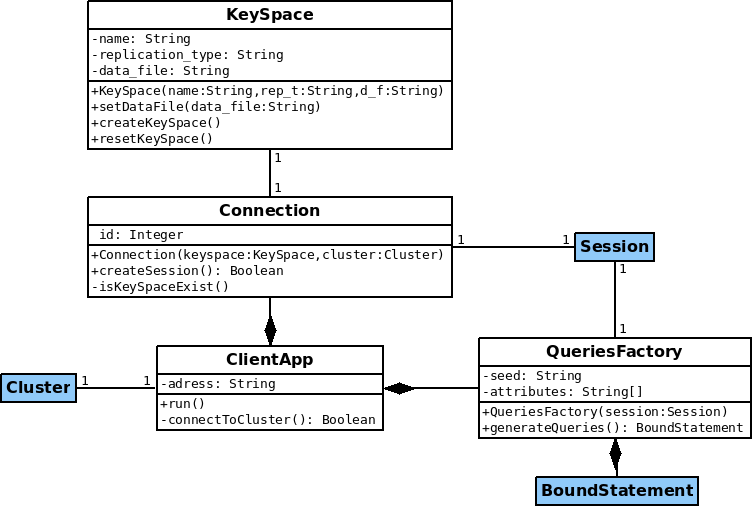
\includegraphics[width=15cm]{schemas/umlclient.png}
	\caption{Diagramme de classe du client. Avec un fond bleu, les classes du pilote \label{fig:umlclient}}
\end{figure}

\subsubsection{ Objet Connection }

\paragraph{} Un \textit{keyspace} est un objet contenant un ensemble de données. C'est l'équivalent d'un \textit{schéma} dans une base de données relationnelle.

\paragraph{} Cet objet permet de créer une session pour exécuter des requêtes dans un keyspace donné.
Si le keyspace n'existe pas, l'objet \path{KeySpace} le crée.

\subsubsection{ Objet KeySpace }

\paragraph{} L'objet \path{KeySpace} permet de créer un keyspace et d'initialiser ses données en fonction d'un jeu de données contenu dans un fichier \path{data_file} écrit au format \path{CQL}.
Si l'utilisateur souhaite importer un autre jeu de données, il suffit de réinitialiser le keyspace avec la méthode \path{resetKeySpace}.

\paragraph{Attributs}
\begin{itemize}
 \item \path{name} : nom du keyspace
 \item \path{replication_type} : choix de l'algorithme d'équilibrage des charges.
 \item \path{data_file} : fichier au format \path{CQL} contenant un jeu de données, suite de requête permettant d'importer des données dans Cassandra.
\end{itemize}


\subsubsection{ Objet QueriesFactory }

\paragraph{} Cet objet permet de génerer ou d'importer des requêtes \path{CQL} que nous exécutons sur une session donnée.

\paragraph{} L'attribut \path{seed} permet la génération de requêtes de manière pseudo-aléatoire. 
Si on change le seed, la suite de requêtes générée sera différente.

\subsubsection{ Objet ClientApp }

\paragraph{} C'est le client, la méthode \path{run} permet de l'exécuter.



\newpage


\section{Visualisation des métriques}

\paragraph{} Pour visualiser les métriques, nous utilisons les applications nommées \path{Graphite} et \path{Cyanite}. Ces applications sont écrites en Python.

\begin{figure}[H]
	\centering
		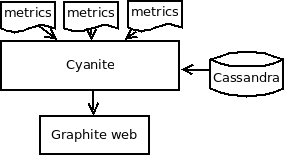
\includegraphics[width=6cm]{schemas/cyanite.png}
	\caption{Architecture pour la visualisation des métriques}
\end{figure}

\paragraph{} Les métriques sont sauvegardées dans des fichiers traités par \path{Cyanite}. 
Puis, \path{Graphite} affiche ces informations sous forme de graphes (courbes, histogrammes...) dans un navigateur web.

\newpage

\bibliography{architecture}

\begin{figure}[p]
	\centering
		% Graphic for TeX using PGF
% Title: C:\Users\Kéké\Pictures\stages.dia
% Creator: Dia v0.97.2
% CreationDate: Sat Feb 14 15:53:37 2015
% For: Kéké
% \usepackage{tikz}
% The following commands are not supported in PSTricks at present
% We define them conditionally, so when they are implemented,
% this pgf file will use them.
\ifx\du\undefined
  \newlength{\du}
\fi
\setlength{\du}{15\unitlength}
\begin{tikzpicture}
\pgftransformxscale{1.000000}
\pgftransformyscale{-1.000000}
\definecolor{dialinecolor}{rgb}{0.000000, 0.000000, 0.000000}
\pgfsetstrokecolor{dialinecolor}
\definecolor{dialinecolor}{rgb}{1.000000, 1.000000, 1.000000}
\pgfsetfillcolor{dialinecolor}
\pgfsetlinewidth{0.100000\du}
\pgfsetdash{}{0pt}
\pgfsetdash{}{0pt}
\pgfsetbuttcap
\pgfsetmiterjoin
\pgfsetlinewidth{0.100000\du}
\pgfsetbuttcap
\pgfsetmiterjoin
\pgfsetdash{}{0pt}
\definecolor{dialinecolor}{rgb}{0.960784, 0.960784, 0.960784}
\pgfsetfillcolor{dialinecolor}
\fill (4.832258\du,6.556250\du)--(4.832258\du,17.476250\du)--(15.400000\du,17.476250\du)--(15.400000\du,6.556250\du)--cycle;
\definecolor{dialinecolor}{rgb}{0.000000, 0.000000, 0.000000}
\pgfsetstrokecolor{dialinecolor}
\draw (4.832258\du,6.556250\du)--(4.832258\du,17.476250\du)--(15.400000\du,17.476250\du)--(15.400000\du,6.556250\du)--cycle;
\pgfsetbuttcap
\pgfsetmiterjoin
\pgfsetdash{}{0pt}
\definecolor{dialinecolor}{rgb}{0.000000, 0.000000, 0.000000}
\pgfsetstrokecolor{dialinecolor}
\draw (4.832258\du,6.556250\du)--(4.832258\du,17.476250\du)--(15.400000\du,17.476250\du)--(15.400000\du,6.556250\du)--cycle;
\pgfsetlinewidth{0.000000\du}
\pgfsetdash{}{0pt}
\pgfsetdash{}{0pt}
\pgfsetbuttcap
\pgfsetmiterjoin
\pgfsetlinewidth{0.000000\du}
\pgfsetbuttcap
\pgfsetmiterjoin
\pgfsetdash{}{0pt}
\definecolor{dialinecolor}{rgb}{0.247059, 0.317647, 0.709804}
\pgfsetfillcolor{dialinecolor}
\fill (1.689994\du,8.035212\du)--(1.689994\du,8.939378\du)--(2.564994\du,8.939378\du)--(2.564994\du,8.035212\du)--cycle;
\definecolor{dialinecolor}{rgb}{0.247059, 0.317647, 0.709804}
\pgfsetstrokecolor{dialinecolor}
\draw (1.689994\du,8.035212\du)--(1.689994\du,8.939378\du)--(2.564994\du,8.939378\du)--(2.564994\du,8.035212\du)--cycle;
\pgfsetbuttcap
\pgfsetmiterjoin
\pgfsetdash{}{0pt}
\definecolor{dialinecolor}{rgb}{0.247059, 0.317647, 0.709804}
\pgfsetstrokecolor{dialinecolor}
\draw (1.689994\du,8.035212\du)--(1.689994\du,8.939378\du)--(2.564994\du,8.939378\du)--(2.564994\du,8.035212\du)--cycle;
\pgfsetlinewidth{0.000000\du}
\pgfsetdash{}{0pt}
\pgfsetdash{}{0pt}
\pgfsetbuttcap
\pgfsetmiterjoin
\pgfsetlinewidth{0.000000\du}
\pgfsetbuttcap
\pgfsetmiterjoin
\pgfsetdash{}{0pt}
\definecolor{dialinecolor}{rgb}{0.247059, 0.317647, 0.709804}
\pgfsetfillcolor{dialinecolor}
\fill (2.844574\du,8.035212\du)--(2.844574\du,8.939379\du)--(3.719574\du,8.939379\du)--(3.719574\du,8.035212\du)--cycle;
\definecolor{dialinecolor}{rgb}{0.247059, 0.317647, 0.709804}
\pgfsetstrokecolor{dialinecolor}
\draw (2.844574\du,8.035212\du)--(2.844574\du,8.939379\du)--(3.719574\du,8.939379\du)--(3.719574\du,8.035212\du)--cycle;
\pgfsetbuttcap
\pgfsetmiterjoin
\pgfsetdash{}{0pt}
\definecolor{dialinecolor}{rgb}{0.247059, 0.317647, 0.709804}
\pgfsetstrokecolor{dialinecolor}
\draw (2.844574\du,8.035212\du)--(2.844574\du,8.939379\du)--(3.719574\du,8.939379\du)--(3.719574\du,8.035212\du)--cycle;
\pgfsetlinewidth{0.000000\du}
\pgfsetdash{}{0pt}
\pgfsetdash{}{0pt}
\pgfsetbuttcap
\pgfsetmiterjoin
\pgfsetlinewidth{0.000000\du}
\pgfsetbuttcap
\pgfsetmiterjoin
\pgfsetdash{}{0pt}
\definecolor{dialinecolor}{rgb}{0.247059, 0.317647, 0.709804}
\pgfsetfillcolor{dialinecolor}
\fill (3.994323\du,8.026865\du)--(3.994323\du,8.931031\du)--(4.869323\du,8.931031\du)--(4.869323\du,8.026865\du)--cycle;
\definecolor{dialinecolor}{rgb}{0.247059, 0.317647, 0.709804}
\pgfsetstrokecolor{dialinecolor}
\draw (3.994323\du,8.026865\du)--(3.994323\du,8.931031\du)--(4.869323\du,8.931031\du)--(4.869323\du,8.026865\du)--cycle;
\pgfsetbuttcap
\pgfsetmiterjoin
\pgfsetdash{}{0pt}
\definecolor{dialinecolor}{rgb}{0.247059, 0.317647, 0.709804}
\pgfsetstrokecolor{dialinecolor}
\draw (3.994323\du,8.026865\du)--(3.994323\du,8.931031\du)--(4.869323\du,8.931031\du)--(4.869323\du,8.026865\du)--cycle;
\pgfsetlinewidth{0.000000\du}
\pgfsetdash{}{0pt}
\pgfsetdash{}{0pt}
\pgfsetbuttcap
\pgfsetmiterjoin
\pgfsetlinewidth{0.000000\du}
\pgfsetbuttcap
\pgfsetmiterjoin
\pgfsetdash{}{0pt}
\definecolor{dialinecolor}{rgb}{0.247059, 0.317647, 0.709804}
\pgfsetfillcolor{dialinecolor}
\fill (5.123068\du,8.033115\du)--(5.123068\du,8.937281\du)--(5.998068\du,8.937281\du)--(5.998068\du,8.033115\du)--cycle;
\definecolor{dialinecolor}{rgb}{0.247059, 0.317647, 0.709804}
\pgfsetstrokecolor{dialinecolor}
\draw (5.123068\du,8.033115\du)--(5.123068\du,8.937281\du)--(5.998068\du,8.937281\du)--(5.998068\du,8.033115\du)--cycle;
\pgfsetbuttcap
\pgfsetmiterjoin
\pgfsetdash{}{0pt}
\definecolor{dialinecolor}{rgb}{0.247059, 0.317647, 0.709804}
\pgfsetstrokecolor{dialinecolor}
\draw (5.123068\du,8.033115\du)--(5.123068\du,8.937281\du)--(5.998068\du,8.937281\du)--(5.998068\du,8.033115\du)--cycle;
\pgfsetlinewidth{0.100000\du}
\pgfsetdash{}{0pt}
\pgfsetdash{}{0pt}
\pgfsetbuttcap
\pgfsetmiterjoin
\pgfsetlinewidth{0.100000\du}
\pgfsetbuttcap
\pgfsetmiterjoin
\pgfsetdash{}{0pt}
\definecolor{dialinecolor}{rgb}{0.247059, 0.317647, 0.709804}
\pgfsetfillcolor{dialinecolor}
\fill (6.388782\du,8.069167\du)--(7.040160\du,8.069167\du)--(7.365849\du,8.484369\du)--(7.040160\du,8.899571\du)--(6.388782\du,8.899571\du)--cycle;
\definecolor{dialinecolor}{rgb}{0.247059, 0.317647, 0.709804}
\pgfsetstrokecolor{dialinecolor}
\draw (6.388782\du,8.069167\du)--(7.040160\du,8.069167\du)--(7.365849\du,8.484369\du)--(7.040160\du,8.899571\du)--(6.388782\du,8.899571\du)--cycle;
\pgfsetbuttcap
\pgfsetmiterjoin
\pgfsetdash{}{0pt}
\definecolor{dialinecolor}{rgb}{0.247059, 0.317647, 0.709804}
\pgfsetstrokecolor{dialinecolor}
\draw (6.388782\du,8.069167\du)--(7.040160\du,8.069167\du)--(7.365849\du,8.484369\du)--(7.040160\du,8.899571\du)--(6.388782\du,8.899571\du)--cycle;
\pgfsetlinewidth{0.100000\du}
\pgfsetdash{}{0pt}
\pgfsetdash{}{0pt}
\pgfsetbuttcap
{
\definecolor{dialinecolor}{rgb}{0.000000, 0.000000, 0.000000}
\pgfsetfillcolor{dialinecolor}
% was here!!!
\pgfsetarrowsend{latex}
\definecolor{dialinecolor}{rgb}{0.000000, 0.000000, 0.000000}
\pgfsetstrokecolor{dialinecolor}
\pgfpathmoveto{\pgfpoint{9.783875\du}{9.050405\du}}
\pgfpatharc{353}{252}{1.549399\du and 1.549399\du}
\pgfusepath{stroke}
}
\definecolor{dialinecolor}{rgb}{1.000000, 1.000000, 1.000000}
\pgfsetfillcolor{dialinecolor}
\pgfpathellipse{\pgfpoint{10.750896\du}{10.500934\du}}{\pgfpoint{3.237421\du}{0\du}}{\pgfpoint{0\du}{1.072133\du}}
\pgfusepath{fill}
\pgfsetlinewidth{0.100000\du}
\pgfsetdash{}{0pt}
\pgfsetdash{}{0pt}
\definecolor{dialinecolor}{rgb}{0.000000, 0.000000, 0.000000}
\pgfsetstrokecolor{dialinecolor}
\pgfpathellipse{\pgfpoint{10.750896\du}{10.500934\du}}{\pgfpoint{3.237421\du}{0\du}}{\pgfpoint{0\du}{1.072133\du}}
\pgfusepath{stroke}
% setfont left to latex
\definecolor{dialinecolor}{rgb}{0.000000, 0.000000, 0.000000}
\pgfsetstrokecolor{dialinecolor}
\node at (10.750896\du,10.314122\du){Traitement};
% setfont left to latex
\definecolor{dialinecolor}{rgb}{0.000000, 0.000000, 0.000000}
\pgfsetstrokecolor{dialinecolor}
\node at (10.750896\du,11.114122\du){de tâche};
\pgfsetlinewidth{0.080000\du}
\pgfsetmiterjoin
\pgfsetdash{}{0pt}
\definecolor{dialinecolor}{rgb}{0.000000, 0.000000, 0.000000}
\pgfsetfillcolor{dialinecolor}
\fill (8.270275\du,13.633244\du)--(8.175675\du,14.276524\du)--(8.610993\du,14.340541\du)--(8.060053\du,15.062754\du)--(8.154653\du,14.419475\du)--(7.719335\du,14.355457\du)--cycle;
\definecolor{dialinecolor}{rgb}{0.000000, 0.000000, 0.000000}
\pgfsetstrokecolor{dialinecolor}
\draw (8.270275\du,13.633244\du)--(8.175675\du,14.276524\du)--(8.610993\du,14.340541\du)--(8.060053\du,15.062754\du)--(8.154653\du,14.419475\du)--(7.719335\du,14.355457\du)--cycle;
\pgfsetlinewidth{0.080000\du}
\pgfsetmiterjoin
\pgfsetdash{}{0pt}
\definecolor{dialinecolor}{rgb}{0.000000, 0.000000, 0.000000}
\pgfsetfillcolor{dialinecolor}
\fill (7.404318\du,13.822444\du)--(7.309718\du,14.465723\du)--(7.745036\du,14.529741\du)--(7.194096\du,15.251954\du)--(7.288696\du,14.608675\du)--(6.853378\du,14.544657\du)--cycle;
\definecolor{dialinecolor}{rgb}{0.000000, 0.000000, 0.000000}
\pgfsetstrokecolor{dialinecolor}
\draw (7.404318\du,13.822444\du)--(7.309718\du,14.465723\du)--(7.745036\du,14.529741\du)--(7.194096\du,15.251954\du)--(7.288696\du,14.608675\du)--(6.853378\du,14.544657\du)--cycle;
\pgfsetlinewidth{0.080000\du}
\pgfsetmiterjoin
\pgfsetdash{}{0pt}
\definecolor{dialinecolor}{rgb}{0.000000, 0.000000, 0.000000}
\pgfsetfillcolor{dialinecolor}
\fill (9.056664\du,14.263910\du)--(8.962064\du,14.907190\du)--(9.397382\du,14.971207\du)--(8.846442\du,15.693421\du)--(8.941042\du,15.050141\du)--(8.505724\du,14.986124\du)--cycle;
\definecolor{dialinecolor}{rgb}{0.000000, 0.000000, 0.000000}
\pgfsetstrokecolor{dialinecolor}
\draw (9.056664\du,14.263910\du)--(8.962064\du,14.907190\du)--(9.397382\du,14.971207\du)--(8.846442\du,15.693421\du)--(8.941042\du,15.050141\du)--(8.505724\du,14.986124\du)--cycle;
\pgfsetlinewidth{0.080000\du}
\pgfsetmiterjoin
\pgfsetdash{}{0pt}
\definecolor{dialinecolor}{rgb}{0.000000, 0.000000, 0.000000}
\pgfsetfillcolor{dialinecolor}
\fill (9.910166\du,13.948577\du)--(9.815566\du,14.591857\du)--(10.250884\du,14.655874\du)--(9.699944\du,15.378088\du)--(9.794544\du,14.734808\du)--(9.359226\du,14.670790\du)--cycle;
\definecolor{dialinecolor}{rgb}{0.000000, 0.000000, 0.000000}
\pgfsetstrokecolor{dialinecolor}
\draw (9.910166\du,13.948577\du)--(9.815566\du,14.591857\du)--(10.250884\du,14.655874\du)--(9.699944\du,15.378088\du)--(9.794544\du,14.734808\du)--(9.359226\du,14.670790\du)--cycle;
\pgfsetlinewidth{0.080000\du}
\pgfsetmiterjoin
\pgfsetdash{}{0pt}
\definecolor{dialinecolor}{rgb}{0.000000, 0.000000, 0.000000}
\pgfsetfillcolor{dialinecolor}
\fill (10.889801\du,14.179821\du)--(10.795201\du,14.823101\du)--(11.230519\du,14.887118\du)--(10.679579\du,15.609332\du)--(10.774179\du,14.966052\du)--(10.338861\du,14.902035\du)--cycle;
\definecolor{dialinecolor}{rgb}{0.000000, 0.000000, 0.000000}
\pgfsetstrokecolor{dialinecolor}
\draw (10.889801\du,14.179821\du)--(10.795201\du,14.823101\du)--(11.230519\du,14.887118\du)--(10.679579\du,15.609332\du)--(10.774179\du,14.966052\du)--(10.338861\du,14.902035\du)--cycle;
\pgfsetlinewidth{0.080000\du}
\pgfsetmiterjoin
\pgfsetdash{}{0pt}
\definecolor{dialinecolor}{rgb}{0.000000, 0.000000, 0.000000}
\pgfsetfillcolor{dialinecolor}
\fill (11.659214\du,13.780399\du)--(11.564614\du,14.423679\du)--(11.999932\du,14.487696\du)--(11.448992\du,15.209910\du)--(11.543592\du,14.566630\du)--(11.108274\du,14.502613\du)--cycle;
\definecolor{dialinecolor}{rgb}{0.000000, 0.000000, 0.000000}
\pgfsetstrokecolor{dialinecolor}
\draw (11.659214\du,13.780399\du)--(11.564614\du,14.423679\du)--(11.999932\du,14.487696\du)--(11.448992\du,15.209910\du)--(11.543592\du,14.566630\du)--(11.108274\du,14.502613\du)--cycle;
\pgfsetlinewidth{0.080000\du}
\pgfsetmiterjoin
\pgfsetdash{}{0pt}
\definecolor{dialinecolor}{rgb}{0.000000, 0.000000, 0.000000}
\pgfsetfillcolor{dialinecolor}
\fill (12.596805\du,13.633244\du)--(12.502205\du,14.276524\du)--(12.937523\du,14.340541\du)--(12.386582\du,15.062754\du)--(12.481182\du,14.419475\du)--(12.045864\du,14.355457\du)--cycle;
\definecolor{dialinecolor}{rgb}{0.000000, 0.000000, 0.000000}
\pgfsetstrokecolor{dialinecolor}
\draw (12.596805\du,13.633244\du)--(12.502205\du,14.276524\du)--(12.937523\du,14.340541\du)--(12.386582\du,15.062754\du)--(12.481182\du,14.419475\du)--(12.045864\du,14.355457\du)--cycle;
% setfont left to latex
\definecolor{dialinecolor}{rgb}{0.000000, 0.000000, 0.000000}
\pgfsetstrokecolor{dialinecolor}
\node[anchor=west] at (4.832258\du,6.406250\du){Stage};
% setfont left to latex
\definecolor{dialinecolor}{rgb}{0.000000, 0.000000, 0.000000}
\pgfsetstrokecolor{dialinecolor}
\node[anchor=west] at (1.689994\du,9.534378\du){File d'attente};
% setfont left to latex
\definecolor{dialinecolor}{rgb}{0.000000, 0.000000, 0.000000}
\pgfsetstrokecolor{dialinecolor}
\node[anchor=west] at (6.584397\du,16.346826\du){Ensemble de threads};
\pgfsetlinewidth{0.100000\du}
\pgfsetdash{}{0pt}
\pgfsetdash{}{0pt}
\pgfsetbuttcap
{
\definecolor{dialinecolor}{rgb}{0.000000, 0.000000, 0.000000}
\pgfsetfillcolor{dialinecolor}
% was here!!!
\pgfsetarrowsend{latex}
\definecolor{dialinecolor}{rgb}{0.000000, 0.000000, 0.000000}
\pgfsetstrokecolor{dialinecolor}
\pgfpathmoveto{\pgfpoint{6.336231\du}{9.933251\du}}
\pgfpatharc{180}{81}{1.589460\du and 1.589460\du}
\pgfusepath{stroke}
}
\pgfsetlinewidth{0.100000\du}
\pgfsetdash{{\pgflinewidth}{0.200000\du}}{0cm}
\pgfsetdash{{\pgflinewidth}{0.200000\du}}{0cm}
\pgfsetbuttcap
{
\definecolor{dialinecolor}{rgb}{0.000000, 0.000000, 0.000000}
\pgfsetfillcolor{dialinecolor}
% was here!!!
\pgfsetarrowsend{latex}
\definecolor{dialinecolor}{rgb}{0.000000, 0.000000, 0.000000}
\pgfsetstrokecolor{dialinecolor}
\draw (7.681653\du,13.591199\du)--(8.985030\du,11.573067\du);
}
\pgfsetlinewidth{0.100000\du}
\pgfsetdash{{\pgflinewidth}{0.200000\du}}{0cm}
\pgfsetdash{{\pgflinewidth}{0.200000\du}}{0cm}
\pgfsetbuttcap
{
\definecolor{dialinecolor}{rgb}{0.000000, 0.000000, 0.000000}
\pgfsetfillcolor{dialinecolor}
% was here!!!
\pgfsetarrowsend{latex}
\definecolor{dialinecolor}{rgb}{0.000000, 0.000000, 0.000000}
\pgfsetstrokecolor{dialinecolor}
\draw (9.571305\du,13.664096\du)--(9.573652\du,11.825334\du);
}
\pgfsetlinewidth{0.100000\du}
\pgfsetdash{{\pgflinewidth}{0.200000\du}}{0cm}
\pgfsetdash{{\pgflinewidth}{0.200000\du}}{0cm}
\pgfsetbuttcap
{
\definecolor{dialinecolor}{rgb}{0.000000, 0.000000, 0.000000}
\pgfsetfillcolor{dialinecolor}
% was here!!!
\pgfsetarrowsend{latex}
\definecolor{dialinecolor}{rgb}{0.000000, 0.000000, 0.000000}
\pgfsetstrokecolor{dialinecolor}
\draw (10.761162\du,13.895341\du)--(10.582718\du,11.993511\du);
}
\pgfsetlinewidth{0.100000\du}
\pgfsetdash{{\pgflinewidth}{0.200000\du}}{0cm}
\pgfsetdash{{\pgflinewidth}{0.200000\du}}{0cm}
\pgfsetbuttcap
{
\definecolor{dialinecolor}{rgb}{0.000000, 0.000000, 0.000000}
\pgfsetfillcolor{dialinecolor}
% was here!!!
\pgfsetarrowsend{latex}
\definecolor{dialinecolor}{rgb}{0.000000, 0.000000, 0.000000}
\pgfsetstrokecolor{dialinecolor}
\draw (11.824886\du,13.495919\du)--(11.633829\du,11.867378\du);
}
\pgfsetlinewidth{0.100000\du}
\pgfsetdash{}{0pt}
\pgfsetdash{}{0pt}
\pgfsetbuttcap
\pgfsetmiterjoin
\pgfsetlinewidth{0.100000\du}
\pgfsetbuttcap
\pgfsetmiterjoin
\pgfsetdash{}{0pt}
\definecolor{dialinecolor}{rgb}{0.960784, 0.960784, 0.960784}
\pgfsetfillcolor{dialinecolor}
\fill (6.768893\du,22.149985\du)--(6.768893\du,33.069985\du)--(17.336635\du,33.069985\du)--(17.336635\du,22.149985\du)--cycle;
\definecolor{dialinecolor}{rgb}{0.000000, 0.000000, 0.000000}
\pgfsetstrokecolor{dialinecolor}
\draw (6.768893\du,22.149985\du)--(6.768893\du,33.069985\du)--(17.336635\du,33.069985\du)--(17.336635\du,22.149985\du)--cycle;
\pgfsetbuttcap
\pgfsetmiterjoin
\pgfsetdash{}{0pt}
\definecolor{dialinecolor}{rgb}{0.000000, 0.000000, 0.000000}
\pgfsetstrokecolor{dialinecolor}
\draw (6.768893\du,22.149985\du)--(6.768893\du,33.069985\du)--(17.336635\du,33.069985\du)--(17.336635\du,22.149985\du)--cycle;
\pgfsetlinewidth{0.000000\du}
\pgfsetdash{}{0pt}
\pgfsetdash{}{0pt}
\pgfsetbuttcap
\pgfsetmiterjoin
\pgfsetlinewidth{0.000000\du}
\pgfsetbuttcap
\pgfsetmiterjoin
\pgfsetdash{}{0pt}
\definecolor{dialinecolor}{rgb}{0.247059, 0.317647, 0.709804}
\pgfsetfillcolor{dialinecolor}
\fill (3.626629\du,23.628947\du)--(3.626629\du,24.533114\du)--(4.501629\du,24.533114\du)--(4.501629\du,23.628947\du)--cycle;
\definecolor{dialinecolor}{rgb}{0.247059, 0.317647, 0.709804}
\pgfsetstrokecolor{dialinecolor}
\draw (3.626629\du,23.628947\du)--(3.626629\du,24.533114\du)--(4.501629\du,24.533114\du)--(4.501629\du,23.628947\du)--cycle;
\pgfsetbuttcap
\pgfsetmiterjoin
\pgfsetdash{}{0pt}
\definecolor{dialinecolor}{rgb}{0.247059, 0.317647, 0.709804}
\pgfsetstrokecolor{dialinecolor}
\draw (3.626629\du,23.628947\du)--(3.626629\du,24.533114\du)--(4.501629\du,24.533114\du)--(4.501629\du,23.628947\du)--cycle;
\pgfsetlinewidth{0.000000\du}
\pgfsetdash{}{0pt}
\pgfsetdash{}{0pt}
\pgfsetbuttcap
\pgfsetmiterjoin
\pgfsetlinewidth{0.000000\du}
\pgfsetbuttcap
\pgfsetmiterjoin
\pgfsetdash{}{0pt}
\definecolor{dialinecolor}{rgb}{0.247059, 0.317647, 0.709804}
\pgfsetfillcolor{dialinecolor}
\fill (4.781209\du,23.628947\du)--(4.781209\du,24.533114\du)--(5.656209\du,24.533114\du)--(5.656209\du,23.628947\du)--cycle;
\definecolor{dialinecolor}{rgb}{0.247059, 0.317647, 0.709804}
\pgfsetstrokecolor{dialinecolor}
\draw (4.781209\du,23.628947\du)--(4.781209\du,24.533114\du)--(5.656209\du,24.533114\du)--(5.656209\du,23.628947\du)--cycle;
\pgfsetbuttcap
\pgfsetmiterjoin
\pgfsetdash{}{0pt}
\definecolor{dialinecolor}{rgb}{0.247059, 0.317647, 0.709804}
\pgfsetstrokecolor{dialinecolor}
\draw (4.781209\du,23.628947\du)--(4.781209\du,24.533114\du)--(5.656209\du,24.533114\du)--(5.656209\du,23.628947\du)--cycle;
\pgfsetlinewidth{0.000000\du}
\pgfsetdash{}{0pt}
\pgfsetdash{}{0pt}
\pgfsetbuttcap
\pgfsetmiterjoin
\pgfsetlinewidth{0.000000\du}
\pgfsetbuttcap
\pgfsetmiterjoin
\pgfsetdash{}{0pt}
\definecolor{dialinecolor}{rgb}{0.247059, 0.317647, 0.709804}
\pgfsetfillcolor{dialinecolor}
\fill (5.930958\du,23.620600\du)--(5.930958\du,24.524767\du)--(6.805958\du,24.524767\du)--(6.805958\du,23.620600\du)--cycle;
\definecolor{dialinecolor}{rgb}{0.247059, 0.317647, 0.709804}
\pgfsetstrokecolor{dialinecolor}
\draw (5.930958\du,23.620600\du)--(5.930958\du,24.524767\du)--(6.805958\du,24.524767\du)--(6.805958\du,23.620600\du)--cycle;
\pgfsetbuttcap
\pgfsetmiterjoin
\pgfsetdash{}{0pt}
\definecolor{dialinecolor}{rgb}{0.247059, 0.317647, 0.709804}
\pgfsetstrokecolor{dialinecolor}
\draw (5.930958\du,23.620600\du)--(5.930958\du,24.524767\du)--(6.805958\du,24.524767\du)--(6.805958\du,23.620600\du)--cycle;
\pgfsetlinewidth{0.000000\du}
\pgfsetdash{}{0pt}
\pgfsetdash{}{0pt}
\pgfsetbuttcap
\pgfsetmiterjoin
\pgfsetlinewidth{0.000000\du}
\pgfsetbuttcap
\pgfsetmiterjoin
\pgfsetdash{}{0pt}
\definecolor{dialinecolor}{rgb}{0.247059, 0.317647, 0.709804}
\pgfsetfillcolor{dialinecolor}
\fill (7.059703\du,23.626850\du)--(7.059703\du,24.531017\du)--(7.934703\du,24.531017\du)--(7.934703\du,23.626850\du)--cycle;
\definecolor{dialinecolor}{rgb}{0.247059, 0.317647, 0.709804}
\pgfsetstrokecolor{dialinecolor}
\draw (7.059703\du,23.626850\du)--(7.059703\du,24.531017\du)--(7.934703\du,24.531017\du)--(7.934703\du,23.626850\du)--cycle;
\pgfsetbuttcap
\pgfsetmiterjoin
\pgfsetdash{}{0pt}
\definecolor{dialinecolor}{rgb}{0.247059, 0.317647, 0.709804}
\pgfsetstrokecolor{dialinecolor}
\draw (7.059703\du,23.626850\du)--(7.059703\du,24.531017\du)--(7.934703\du,24.531017\du)--(7.934703\du,23.626850\du)--cycle;
\pgfsetlinewidth{0.100000\du}
\pgfsetdash{}{0pt}
\pgfsetdash{}{0pt}
\pgfsetbuttcap
\pgfsetmiterjoin
\pgfsetlinewidth{0.100000\du}
\pgfsetbuttcap
\pgfsetmiterjoin
\pgfsetdash{}{0pt}
\definecolor{dialinecolor}{rgb}{0.247059, 0.317647, 0.709804}
\pgfsetfillcolor{dialinecolor}
\fill (8.325417\du,23.662902\du)--(8.976795\du,23.662902\du)--(9.302484\du,24.078104\du)--(8.976795\du,24.493306\du)--(8.325417\du,24.493306\du)--cycle;
\definecolor{dialinecolor}{rgb}{0.247059, 0.317647, 0.709804}
\pgfsetstrokecolor{dialinecolor}
\draw (8.325417\du,23.662902\du)--(8.976795\du,23.662902\du)--(9.302484\du,24.078104\du)--(8.976795\du,24.493306\du)--(8.325417\du,24.493306\du)--cycle;
\pgfsetbuttcap
\pgfsetmiterjoin
\pgfsetdash{}{0pt}
\definecolor{dialinecolor}{rgb}{0.247059, 0.317647, 0.709804}
\pgfsetstrokecolor{dialinecolor}
\draw (8.325417\du,23.662902\du)--(8.976795\du,23.662902\du)--(9.302484\du,24.078104\du)--(8.976795\du,24.493306\du)--(8.325417\du,24.493306\du)--cycle;
\pgfsetlinewidth{0.100000\du}
\pgfsetdash{}{0pt}
\pgfsetdash{}{0pt}
\pgfsetbuttcap
{
\definecolor{dialinecolor}{rgb}{0.000000, 0.000000, 0.000000}
\pgfsetfillcolor{dialinecolor}
% was here!!!
\pgfsetarrowsend{latex}
\definecolor{dialinecolor}{rgb}{0.000000, 0.000000, 0.000000}
\pgfsetstrokecolor{dialinecolor}
\pgfpathmoveto{\pgfpoint{11.720510\du}{24.644140\du}}
\pgfpatharc{353}{252}{1.549399\du and 1.549399\du}
\pgfusepath{stroke}
}
\definecolor{dialinecolor}{rgb}{1.000000, 1.000000, 1.000000}
\pgfsetfillcolor{dialinecolor}
\pgfpathellipse{\pgfpoint{12.687531\du}{26.094669\du}}{\pgfpoint{3.237421\du}{0\du}}{\pgfpoint{0\du}{1.072133\du}}
\pgfusepath{fill}
\pgfsetlinewidth{0.100000\du}
\pgfsetdash{}{0pt}
\pgfsetdash{}{0pt}
\definecolor{dialinecolor}{rgb}{0.000000, 0.000000, 0.000000}
\pgfsetstrokecolor{dialinecolor}
\pgfpathellipse{\pgfpoint{12.687531\du}{26.094669\du}}{\pgfpoint{3.237421\du}{0\du}}{\pgfpoint{0\du}{1.072133\du}}
\pgfusepath{stroke}
% setfont left to latex
\definecolor{dialinecolor}{rgb}{0.000000, 0.000000, 0.000000}
\pgfsetstrokecolor{dialinecolor}
\node at (12.687531\du,25.917169\du){Traitement};
% setfont left to latex
\definecolor{dialinecolor}{rgb}{0.000000, 0.000000, 0.000000}
\pgfsetstrokecolor{dialinecolor}
\node at (12.687531\du,26.717169\du){de tâche};
\pgfsetlinewidth{0.080000\du}
\pgfsetmiterjoin
\pgfsetdash{}{0pt}
\definecolor{dialinecolor}{rgb}{0.000000, 0.000000, 0.000000}
\pgfsetfillcolor{dialinecolor}
\fill (10.206910\du,29.226979\du)--(10.112310\du,29.870259\du)--(10.547628\du,29.934276\du)--(9.996688\du,30.656489\du)--(10.091288\du,30.013210\du)--(9.655970\du,29.949192\du)--cycle;
\definecolor{dialinecolor}{rgb}{0.000000, 0.000000, 0.000000}
\pgfsetstrokecolor{dialinecolor}
\draw (10.206910\du,29.226979\du)--(10.112310\du,29.870259\du)--(10.547628\du,29.934276\du)--(9.996688\du,30.656489\du)--(10.091288\du,30.013210\du)--(9.655970\du,29.949192\du)--cycle;
\pgfsetlinewidth{0.080000\du}
\pgfsetmiterjoin
\pgfsetdash{}{0pt}
\definecolor{dialinecolor}{rgb}{0.000000, 0.000000, 0.000000}
\pgfsetfillcolor{dialinecolor}
\fill (9.340953\du,29.416179\du)--(9.246353\du,30.059459\du)--(9.681671\du,30.123476\du)--(9.130731\du,30.845689\du)--(9.225331\du,30.202410\du)--(8.790013\du,30.138392\du)--cycle;
\definecolor{dialinecolor}{rgb}{0.000000, 0.000000, 0.000000}
\pgfsetstrokecolor{dialinecolor}
\draw (9.340953\du,29.416179\du)--(9.246353\du,30.059459\du)--(9.681671\du,30.123476\du)--(9.130731\du,30.845689\du)--(9.225331\du,30.202410\du)--(8.790013\du,30.138392\du)--cycle;
\pgfsetlinewidth{0.080000\du}
\pgfsetmiterjoin
\pgfsetdash{}{0pt}
\definecolor{dialinecolor}{rgb}{0.000000, 0.000000, 0.000000}
\pgfsetfillcolor{dialinecolor}
\fill (10.993299\du,29.857645\du)--(10.898699\du,30.500925\du)--(11.334017\du,30.564942\du)--(10.783077\du,31.287156\du)--(10.877677\du,30.643876\du)--(10.442359\du,30.579859\du)--cycle;
\definecolor{dialinecolor}{rgb}{0.000000, 0.000000, 0.000000}
\pgfsetstrokecolor{dialinecolor}
\draw (10.993299\du,29.857645\du)--(10.898699\du,30.500925\du)--(11.334017\du,30.564942\du)--(10.783077\du,31.287156\du)--(10.877677\du,30.643876\du)--(10.442359\du,30.579859\du)--cycle;
\pgfsetlinewidth{0.080000\du}
\pgfsetmiterjoin
\pgfsetdash{}{0pt}
\definecolor{dialinecolor}{rgb}{0.000000, 0.000000, 0.000000}
\pgfsetfillcolor{dialinecolor}
\fill (11.846801\du,29.542312\du)--(11.752201\du,30.185592\du)--(12.187519\du,30.249609\du)--(11.636579\du,30.971823\du)--(11.731179\du,30.328543\du)--(11.295861\du,30.264526\du)--cycle;
\definecolor{dialinecolor}{rgb}{0.000000, 0.000000, 0.000000}
\pgfsetstrokecolor{dialinecolor}
\draw (11.846801\du,29.542312\du)--(11.752201\du,30.185592\du)--(12.187519\du,30.249609\du)--(11.636579\du,30.971823\du)--(11.731179\du,30.328543\du)--(11.295861\du,30.264526\du)--cycle;
\pgfsetlinewidth{0.080000\du}
\pgfsetmiterjoin
\pgfsetdash{}{0pt}
\definecolor{dialinecolor}{rgb}{0.000000, 0.000000, 0.000000}
\pgfsetfillcolor{dialinecolor}
\fill (12.826436\du,29.773557\du)--(12.731836\du,30.416836\du)--(13.167154\du,30.480854\du)--(12.616214\du,31.203067\du)--(12.710814\du,30.559787\du)--(12.275496\du,30.495770\du)--cycle;
\definecolor{dialinecolor}{rgb}{0.000000, 0.000000, 0.000000}
\pgfsetstrokecolor{dialinecolor}
\draw (12.826436\du,29.773557\du)--(12.731836\du,30.416836\du)--(13.167154\du,30.480854\du)--(12.616214\du,31.203067\du)--(12.710814\du,30.559787\du)--(12.275496\du,30.495770\du)--cycle;
\pgfsetlinewidth{0.080000\du}
\pgfsetmiterjoin
\pgfsetdash{}{0pt}
\definecolor{dialinecolor}{rgb}{0.000000, 0.000000, 0.000000}
\pgfsetfillcolor{dialinecolor}
\fill (13.595849\du,29.374134\du)--(13.501249\du,30.017414\du)--(13.936567\du,30.081432\du)--(13.385627\du,30.803645\du)--(13.480227\du,30.160365\du)--(13.044909\du,30.096348\du)--cycle;
\definecolor{dialinecolor}{rgb}{0.000000, 0.000000, 0.000000}
\pgfsetstrokecolor{dialinecolor}
\draw (13.595849\du,29.374134\du)--(13.501249\du,30.017414\du)--(13.936567\du,30.081432\du)--(13.385627\du,30.803645\du)--(13.480227\du,30.160365\du)--(13.044909\du,30.096348\du)--cycle;
\pgfsetlinewidth{0.080000\du}
\pgfsetmiterjoin
\pgfsetdash{}{0pt}
\definecolor{dialinecolor}{rgb}{0.000000, 0.000000, 0.000000}
\pgfsetfillcolor{dialinecolor}
\fill (14.533440\du,29.226979\du)--(14.438840\du,29.870259\du)--(14.874158\du,29.934276\du)--(14.323218\du,30.656489\du)--(14.417817\du,30.013210\du)--(13.982499\du,29.949192\du)--cycle;
\definecolor{dialinecolor}{rgb}{0.000000, 0.000000, 0.000000}
\pgfsetstrokecolor{dialinecolor}
\draw (14.533440\du,29.226979\du)--(14.438840\du,29.870259\du)--(14.874158\du,29.934276\du)--(14.323218\du,30.656489\du)--(14.417817\du,30.013210\du)--(13.982499\du,29.949192\du)--cycle;
% setfont left to latex
\definecolor{dialinecolor}{rgb}{0.000000, 0.000000, 0.000000}
\pgfsetstrokecolor{dialinecolor}
\node[anchor=west] at (6.768893\du,21.999985\du){Stage};
% setfont left to latex
\definecolor{dialinecolor}{rgb}{0.000000, 0.000000, 0.000000}
\pgfsetstrokecolor{dialinecolor}
\node[anchor=west] at (3.626629\du,25.128114\du){File d'attente};
% setfont left to latex
\definecolor{dialinecolor}{rgb}{0.000000, 0.000000, 0.000000}
\pgfsetstrokecolor{dialinecolor}
\node[anchor=west] at (8.521032\du,31.940561\du){Ensemble de threads};
\pgfsetlinewidth{0.100000\du}
\pgfsetdash{}{0pt}
\pgfsetdash{}{0pt}
\pgfsetbuttcap
{
\definecolor{dialinecolor}{rgb}{0.000000, 0.000000, 0.000000}
\pgfsetfillcolor{dialinecolor}
% was here!!!
\pgfsetarrowsend{latex}
\definecolor{dialinecolor}{rgb}{0.000000, 0.000000, 0.000000}
\pgfsetstrokecolor{dialinecolor}
\pgfpathmoveto{\pgfpoint{8.272866\du}{25.526986\du}}
\pgfpatharc{180}{81}{1.589460\du and 1.589460\du}
\pgfusepath{stroke}
}
\pgfsetlinewidth{0.100000\du}
\pgfsetdash{{\pgflinewidth}{0.200000\du}}{0cm}
\pgfsetdash{{\pgflinewidth}{0.200000\du}}{0cm}
\pgfsetbuttcap
{
\definecolor{dialinecolor}{rgb}{0.000000, 0.000000, 0.000000}
\pgfsetfillcolor{dialinecolor}
% was here!!!
\pgfsetarrowsend{latex}
\definecolor{dialinecolor}{rgb}{0.000000, 0.000000, 0.000000}
\pgfsetstrokecolor{dialinecolor}
\draw (9.618288\du,29.184935\du)--(10.921665\du,27.166802\du);
}
\pgfsetlinewidth{0.100000\du}
\pgfsetdash{{\pgflinewidth}{0.200000\du}}{0cm}
\pgfsetdash{{\pgflinewidth}{0.200000\du}}{0cm}
\pgfsetbuttcap
{
\definecolor{dialinecolor}{rgb}{0.000000, 0.000000, 0.000000}
\pgfsetfillcolor{dialinecolor}
% was here!!!
\pgfsetarrowsend{latex}
\definecolor{dialinecolor}{rgb}{0.000000, 0.000000, 0.000000}
\pgfsetstrokecolor{dialinecolor}
\draw (11.507940\du,29.257832\du)--(11.510287\du,27.419069\du);
}
\pgfsetlinewidth{0.100000\du}
\pgfsetdash{{\pgflinewidth}{0.200000\du}}{0cm}
\pgfsetdash{{\pgflinewidth}{0.200000\du}}{0cm}
\pgfsetbuttcap
{
\definecolor{dialinecolor}{rgb}{0.000000, 0.000000, 0.000000}
\pgfsetfillcolor{dialinecolor}
% was here!!!
\pgfsetarrowsend{latex}
\definecolor{dialinecolor}{rgb}{0.000000, 0.000000, 0.000000}
\pgfsetstrokecolor{dialinecolor}
\draw (12.697797\du,29.489076\du)--(12.519353\du,27.587246\du);
}
\pgfsetlinewidth{0.100000\du}
\pgfsetdash{{\pgflinewidth}{0.200000\du}}{0cm}
\pgfsetdash{{\pgflinewidth}{0.200000\du}}{0cm}
\pgfsetbuttcap
{
\definecolor{dialinecolor}{rgb}{0.000000, 0.000000, 0.000000}
\pgfsetfillcolor{dialinecolor}
% was here!!!
\pgfsetarrowsend{latex}
\definecolor{dialinecolor}{rgb}{0.000000, 0.000000, 0.000000}
\pgfsetstrokecolor{dialinecolor}
\draw (13.761521\du,29.089654\du)--(13.570464\du,27.461113\du);
}
\pgfsetlinewidth{0.200000\du}
\pgfsetdash{}{0pt}
\pgfsetdash{}{0pt}
\pgfsetmiterjoin
\pgfsetbuttcap
{
\definecolor{dialinecolor}{rgb}{0.000000, 0.000000, 0.000000}
\pgfsetfillcolor{dialinecolor}
% was here!!!
\pgfsetarrowsend{latex}
\definecolor{dialinecolor}{rgb}{0.000000, 0.000000, 0.000000}
\pgfsetstrokecolor{dialinecolor}
\pgfpathmoveto{\pgfpoint{13.988317\du}{10.500934\du}}
\pgfpathcurveto{\pgfpoint{18.441040\du}{10.922577\du}}{\pgfpoint{21.439908\du}{10.759002\du}}{\pgfpoint{21.167284\du}{15.502667\du}}
\pgfpathcurveto{\pgfpoint{20.894660\du}{20.246331\du}}{\pgfpoint{10.044208\du}{20.191807\du}}{\pgfpoint{6.336516\du}{20.137282\du}}
\pgfpathcurveto{\pgfpoint{2.628824\du}{20.082757\du}}{\pgfpoint{0.175204\du}{24.390222\du}}{\pgfpoint{3.626629\du}{24.081030\du}}
\pgfusepath{stroke}
}
% setfont left to latex
\definecolor{dialinecolor}{rgb}{0.000000, 0.000000, 0.000000}
\pgfsetstrokecolor{dialinecolor}
\node[anchor=west] at (16.423619\du,10.540902\du){Nouvelle tâche};
\end{tikzpicture}

	\caption{Schéma de deux stages dans une architecture SEDA \label{fig:stages}}
\end{figure}

\begin{figure}[p]
	\centering
		% Graphic for TeX using PGF
% Title: C:\Users\Kéké\Pictures\read_request.dia
% Creator: Dia v0.97.2
% CreationDate: Sat Feb 14 17:33:20 2015
% For: Kéké
% \usepackage{tikz}
% The following commands are not supported in PSTricks at present
% We define them conditionally, so when they are implemented,
% this pgf file will use them.
\ifx\du\undefined
  \newlength{\du}
\fi
\setlength{\du}{15\unitlength}
\begin{tikzpicture}
\pgftransformxscale{1.000000}
\pgftransformyscale{-1.000000}
\definecolor{dialinecolor}{rgb}{0.000000, 0.000000, 0.000000}
\pgfsetstrokecolor{dialinecolor}
\definecolor{dialinecolor}{rgb}{1.000000, 1.000000, 1.000000}
\pgfsetfillcolor{dialinecolor}
\pgfsetlinewidth{0.100000\du}
\pgfsetdash{}{0pt}
\pgfsetdash{}{0pt}
\pgfsetbuttcap
\pgfsetmiterjoin
\pgfsetlinewidth{0.100000\du}
\pgfsetbuttcap
\pgfsetmiterjoin
\pgfsetdash{}{0pt}
\definecolor{dialinecolor}{rgb}{0.960784, 0.960784, 0.960784}
\pgfsetfillcolor{dialinecolor}
\fill (16.427264\du,15.075001\du)--(16.427264\du,21.782215\du)--(22.918116\du,21.782215\du)--(22.918116\du,15.075001\du)--cycle;
\definecolor{dialinecolor}{rgb}{0.000000, 0.000000, 0.000000}
\pgfsetstrokecolor{dialinecolor}
\draw (16.427264\du,15.075001\du)--(16.427264\du,21.782215\du)--(22.918116\du,21.782215\du)--(22.918116\du,15.075001\du)--cycle;
\pgfsetbuttcap
\pgfsetmiterjoin
\pgfsetdash{}{0pt}
\definecolor{dialinecolor}{rgb}{0.000000, 0.000000, 0.000000}
\pgfsetstrokecolor{dialinecolor}
\draw (16.427264\du,15.075001\du)--(16.427264\du,21.782215\du)--(22.918116\du,21.782215\du)--(22.918116\du,15.075001\du)--cycle;
\pgfsetlinewidth{0.000000\du}
\pgfsetdash{}{0pt}
\pgfsetdash{}{0pt}
\pgfsetbuttcap
\pgfsetmiterjoin
\pgfsetlinewidth{0.000000\du}
\pgfsetbuttcap
\pgfsetmiterjoin
\pgfsetdash{}{0pt}
\definecolor{dialinecolor}{rgb}{0.247059, 0.317647, 0.709804}
\pgfsetfillcolor{dialinecolor}
\fill (15.235000\du,16.703963\du)--(15.235000\du,17.608130\du)--(16.110000\du,17.608130\du)--(16.110000\du,16.703963\du)--cycle;
\definecolor{dialinecolor}{rgb}{0.247059, 0.317647, 0.709804}
\pgfsetstrokecolor{dialinecolor}
\draw (15.235000\du,16.703963\du)--(15.235000\du,17.608130\du)--(16.110000\du,17.608130\du)--(16.110000\du,16.703963\du)--cycle;
\pgfsetbuttcap
\pgfsetmiterjoin
\pgfsetdash{}{0pt}
\definecolor{dialinecolor}{rgb}{0.247059, 0.317647, 0.709804}
\pgfsetstrokecolor{dialinecolor}
\draw (15.235000\du,16.703963\du)--(15.235000\du,17.608130\du)--(16.110000\du,17.608130\du)--(16.110000\du,16.703963\du)--cycle;
\pgfsetlinewidth{0.000000\du}
\pgfsetdash{}{0pt}
\pgfsetdash{}{0pt}
\pgfsetbuttcap
\pgfsetmiterjoin
\pgfsetlinewidth{0.000000\du}
\pgfsetbuttcap
\pgfsetmiterjoin
\pgfsetdash{}{0pt}
\definecolor{dialinecolor}{rgb}{0.247059, 0.317647, 0.709804}
\pgfsetfillcolor{dialinecolor}
\fill (16.389580\du,16.703963\du)--(16.389580\du,17.608130\du)--(17.264580\du,17.608130\du)--(17.264580\du,16.703963\du)--cycle;
\definecolor{dialinecolor}{rgb}{0.247059, 0.317647, 0.709804}
\pgfsetstrokecolor{dialinecolor}
\draw (16.389580\du,16.703963\du)--(16.389580\du,17.608130\du)--(17.264580\du,17.608130\du)--(17.264580\du,16.703963\du)--cycle;
\pgfsetbuttcap
\pgfsetmiterjoin
\pgfsetdash{}{0pt}
\definecolor{dialinecolor}{rgb}{0.247059, 0.317647, 0.709804}
\pgfsetstrokecolor{dialinecolor}
\draw (16.389580\du,16.703963\du)--(16.389580\du,17.608130\du)--(17.264580\du,17.608130\du)--(17.264580\du,16.703963\du)--cycle;
\pgfsetlinewidth{0.000000\du}
\pgfsetdash{}{0pt}
\pgfsetdash{}{0pt}
\pgfsetbuttcap
\pgfsetmiterjoin
\pgfsetlinewidth{0.000000\du}
\pgfsetbuttcap
\pgfsetmiterjoin
\pgfsetdash{}{0pt}
\definecolor{dialinecolor}{rgb}{0.247059, 0.317647, 0.709804}
\pgfsetfillcolor{dialinecolor}
\fill (17.539328\du,16.695616\du)--(17.539328\du,17.599783\du)--(18.414328\du,17.599783\du)--(18.414328\du,16.695616\du)--cycle;
\definecolor{dialinecolor}{rgb}{0.247059, 0.317647, 0.709804}
\pgfsetstrokecolor{dialinecolor}
\draw (17.539328\du,16.695616\du)--(17.539328\du,17.599783\du)--(18.414328\du,17.599783\du)--(18.414328\du,16.695616\du)--cycle;
\pgfsetbuttcap
\pgfsetmiterjoin
\pgfsetdash{}{0pt}
\definecolor{dialinecolor}{rgb}{0.247059, 0.317647, 0.709804}
\pgfsetstrokecolor{dialinecolor}
\draw (17.539328\du,16.695616\du)--(17.539328\du,17.599783\du)--(18.414328\du,17.599783\du)--(18.414328\du,16.695616\du)--cycle;
\pgfsetlinewidth{0.000000\du}
\pgfsetdash{}{0pt}
\pgfsetdash{}{0pt}
\pgfsetbuttcap
\pgfsetmiterjoin
\pgfsetlinewidth{0.000000\du}
\pgfsetbuttcap
\pgfsetmiterjoin
\pgfsetdash{}{0pt}
\definecolor{dialinecolor}{rgb}{0.247059, 0.317647, 0.709804}
\pgfsetfillcolor{dialinecolor}
\fill (18.668074\du,16.701866\du)--(18.668074\du,17.606033\du)--(19.543074\du,17.606033\du)--(19.543074\du,16.701866\du)--cycle;
\definecolor{dialinecolor}{rgb}{0.247059, 0.317647, 0.709804}
\pgfsetstrokecolor{dialinecolor}
\draw (18.668074\du,16.701866\du)--(18.668074\du,17.606033\du)--(19.543074\du,17.606033\du)--(19.543074\du,16.701866\du)--cycle;
\pgfsetbuttcap
\pgfsetmiterjoin
\pgfsetdash{}{0pt}
\definecolor{dialinecolor}{rgb}{0.247059, 0.317647, 0.709804}
\pgfsetstrokecolor{dialinecolor}
\draw (18.668074\du,16.701866\du)--(18.668074\du,17.606033\du)--(19.543074\du,17.606033\du)--(19.543074\du,16.701866\du)--cycle;
\pgfsetlinewidth{0.100000\du}
\pgfsetdash{}{0pt}
\pgfsetdash{}{0pt}
\pgfsetbuttcap
\pgfsetmiterjoin
\pgfsetlinewidth{0.100000\du}
\pgfsetbuttcap
\pgfsetmiterjoin
\pgfsetdash{}{0pt}
\definecolor{dialinecolor}{rgb}{0.247059, 0.317647, 0.709804}
\pgfsetfillcolor{dialinecolor}
\fill (19.933787\du,16.737918\du)--(20.585166\du,16.737918\du)--(20.910855\du,17.153120\du)--(20.585166\du,17.568322\du)--(19.933787\du,17.568322\du)--cycle;
\definecolor{dialinecolor}{rgb}{0.247059, 0.317647, 0.709804}
\pgfsetstrokecolor{dialinecolor}
\draw (19.933787\du,16.737918\du)--(20.585166\du,16.737918\du)--(20.910855\du,17.153120\du)--(20.585166\du,17.568322\du)--(19.933787\du,17.568322\du)--cycle;
\pgfsetbuttcap
\pgfsetmiterjoin
\pgfsetdash{}{0pt}
\definecolor{dialinecolor}{rgb}{0.247059, 0.317647, 0.709804}
\pgfsetstrokecolor{dialinecolor}
\draw (19.933787\du,16.737918\du)--(20.585166\du,16.737918\du)--(20.910855\du,17.153120\du)--(20.585166\du,17.568322\du)--(19.933787\du,17.568322\du)--cycle;
% setfont left to latex
\definecolor{dialinecolor}{rgb}{0.000000, 0.000000, 0.000000}
\pgfsetstrokecolor{dialinecolor}
\node[anchor=west] at (16.427264\du,14.895001\du){QueueManagerStage};
% setfont left to latex
\definecolor{dialinecolor}{rgb}{0.000000, 0.000000, 0.000000}
\pgfsetstrokecolor{dialinecolor}
\node[anchor=west] at (15.235000\du,18.203130\du){File d'attente};
% setfont left to latex
\definecolor{dialinecolor}{rgb}{1.000000, 0.341176, 0.133333}
\pgfsetstrokecolor{dialinecolor}
\node[anchor=west] at (20.211135\du,16.035002\du){Node 2};
\pgfsetlinewidth{0.100000\du}
\pgfsetdash{}{0pt}
\pgfsetdash{}{0pt}
\pgfsetbuttcap
\pgfsetmiterjoin
\pgfsetlinewidth{0.100000\du}
\pgfsetbuttcap
\pgfsetmiterjoin
\pgfsetdash{}{0pt}
\definecolor{dialinecolor}{rgb}{0.960784, 0.960784, 0.960784}
\pgfsetfillcolor{dialinecolor}
\fill (7.327366\du,5.325003\du)--(7.327366\du,12.032217\du)--(13.818218\du,12.032217\du)--(13.818218\du,5.325003\du)--cycle;
\definecolor{dialinecolor}{rgb}{0.000000, 0.000000, 0.000000}
\pgfsetstrokecolor{dialinecolor}
\draw (7.327366\du,5.325003\du)--(7.327366\du,12.032217\du)--(13.818218\du,12.032217\du)--(13.818218\du,5.325003\du)--cycle;
\pgfsetbuttcap
\pgfsetmiterjoin
\pgfsetdash{}{0pt}
\definecolor{dialinecolor}{rgb}{0.000000, 0.000000, 0.000000}
\pgfsetstrokecolor{dialinecolor}
\draw (7.327366\du,5.325003\du)--(7.327366\du,12.032217\du)--(13.818218\du,12.032217\du)--(13.818218\du,5.325003\du)--cycle;
\pgfsetlinewidth{0.000000\du}
\pgfsetdash{}{0pt}
\pgfsetdash{}{0pt}
\pgfsetbuttcap
\pgfsetmiterjoin
\pgfsetlinewidth{0.000000\du}
\pgfsetbuttcap
\pgfsetmiterjoin
\pgfsetdash{}{0pt}
\definecolor{dialinecolor}{rgb}{0.247059, 0.317647, 0.709804}
\pgfsetfillcolor{dialinecolor}
\fill (6.135102\du,6.953965\du)--(6.135102\du,7.858131\du)--(7.010102\du,7.858131\du)--(7.010102\du,6.953965\du)--cycle;
\definecolor{dialinecolor}{rgb}{0.247059, 0.317647, 0.709804}
\pgfsetstrokecolor{dialinecolor}
\draw (6.135102\du,6.953965\du)--(6.135102\du,7.858131\du)--(7.010102\du,7.858131\du)--(7.010102\du,6.953965\du)--cycle;
\pgfsetbuttcap
\pgfsetmiterjoin
\pgfsetdash{}{0pt}
\definecolor{dialinecolor}{rgb}{0.247059, 0.317647, 0.709804}
\pgfsetstrokecolor{dialinecolor}
\draw (6.135102\du,6.953965\du)--(6.135102\du,7.858131\du)--(7.010102\du,7.858131\du)--(7.010102\du,6.953965\du)--cycle;
\pgfsetlinewidth{0.000000\du}
\pgfsetdash{}{0pt}
\pgfsetdash{}{0pt}
\pgfsetbuttcap
\pgfsetmiterjoin
\pgfsetlinewidth{0.000000\du}
\pgfsetbuttcap
\pgfsetmiterjoin
\pgfsetdash{}{0pt}
\definecolor{dialinecolor}{rgb}{0.247059, 0.317647, 0.709804}
\pgfsetfillcolor{dialinecolor}
\fill (7.289682\du,6.953965\du)--(7.289682\du,7.858132\du)--(8.164682\du,7.858132\du)--(8.164682\du,6.953965\du)--cycle;
\definecolor{dialinecolor}{rgb}{0.247059, 0.317647, 0.709804}
\pgfsetstrokecolor{dialinecolor}
\draw (7.289682\du,6.953965\du)--(7.289682\du,7.858132\du)--(8.164682\du,7.858132\du)--(8.164682\du,6.953965\du)--cycle;
\pgfsetbuttcap
\pgfsetmiterjoin
\pgfsetdash{}{0pt}
\definecolor{dialinecolor}{rgb}{0.247059, 0.317647, 0.709804}
\pgfsetstrokecolor{dialinecolor}
\draw (7.289682\du,6.953965\du)--(7.289682\du,7.858132\du)--(8.164682\du,7.858132\du)--(8.164682\du,6.953965\du)--cycle;
\pgfsetlinewidth{0.000000\du}
\pgfsetdash{}{0pt}
\pgfsetdash{}{0pt}
\pgfsetbuttcap
\pgfsetmiterjoin
\pgfsetlinewidth{0.000000\du}
\pgfsetbuttcap
\pgfsetmiterjoin
\pgfsetdash{}{0pt}
\definecolor{dialinecolor}{rgb}{0.611765, 0.152941, 0.690196}
\pgfsetfillcolor{dialinecolor}
\fill (8.439430\du,6.945618\du)--(8.439430\du,7.849784\du)--(9.314430\du,7.849784\du)--(9.314430\du,6.945618\du)--cycle;
\definecolor{dialinecolor}{rgb}{0.611765, 0.152941, 0.690196}
\pgfsetstrokecolor{dialinecolor}
\draw (8.439430\du,6.945618\du)--(8.439430\du,7.849784\du)--(9.314430\du,7.849784\du)--(9.314430\du,6.945618\du)--cycle;
\pgfsetbuttcap
\pgfsetmiterjoin
\pgfsetdash{}{0pt}
\definecolor{dialinecolor}{rgb}{0.611765, 0.152941, 0.690196}
\pgfsetstrokecolor{dialinecolor}
\draw (8.439430\du,6.945618\du)--(8.439430\du,7.849784\du)--(9.314430\du,7.849784\du)--(9.314430\du,6.945618\du)--cycle;
\pgfsetlinewidth{0.000000\du}
\pgfsetdash{}{0pt}
\pgfsetdash{}{0pt}
\pgfsetbuttcap
\pgfsetmiterjoin
\pgfsetlinewidth{0.000000\du}
\pgfsetbuttcap
\pgfsetmiterjoin
\pgfsetdash{}{0pt}
\definecolor{dialinecolor}{rgb}{0.247059, 0.317647, 0.709804}
\pgfsetfillcolor{dialinecolor}
\fill (9.568176\du,6.951868\du)--(9.568176\du,7.856034\du)--(10.443176\du,7.856034\du)--(10.443176\du,6.951868\du)--cycle;
\definecolor{dialinecolor}{rgb}{0.247059, 0.317647, 0.709804}
\pgfsetstrokecolor{dialinecolor}
\draw (9.568176\du,6.951868\du)--(9.568176\du,7.856034\du)--(10.443176\du,7.856034\du)--(10.443176\du,6.951868\du)--cycle;
\pgfsetbuttcap
\pgfsetmiterjoin
\pgfsetdash{}{0pt}
\definecolor{dialinecolor}{rgb}{0.247059, 0.317647, 0.709804}
\pgfsetstrokecolor{dialinecolor}
\draw (9.568176\du,6.951868\du)--(9.568176\du,7.856034\du)--(10.443176\du,7.856034\du)--(10.443176\du,6.951868\du)--cycle;
\pgfsetlinewidth{0.100000\du}
\pgfsetdash{}{0pt}
\pgfsetdash{}{0pt}
\pgfsetbuttcap
\pgfsetmiterjoin
\pgfsetlinewidth{0.100000\du}
\pgfsetbuttcap
\pgfsetmiterjoin
\pgfsetdash{}{0pt}
\definecolor{dialinecolor}{rgb}{0.247059, 0.317647, 0.709804}
\pgfsetfillcolor{dialinecolor}
\fill (10.833889\du,6.987920\du)--(11.485267\du,6.987920\du)--(11.810957\du,7.403122\du)--(11.485267\du,7.818324\du)--(10.833889\du,7.818324\du)--cycle;
\definecolor{dialinecolor}{rgb}{0.247059, 0.317647, 0.709804}
\pgfsetstrokecolor{dialinecolor}
\draw (10.833889\du,6.987920\du)--(11.485267\du,6.987920\du)--(11.810957\du,7.403122\du)--(11.485267\du,7.818324\du)--(10.833889\du,7.818324\du)--cycle;
\pgfsetbuttcap
\pgfsetmiterjoin
\pgfsetdash{}{0pt}
\definecolor{dialinecolor}{rgb}{0.247059, 0.317647, 0.709804}
\pgfsetstrokecolor{dialinecolor}
\draw (10.833889\du,6.987920\du)--(11.485267\du,6.987920\du)--(11.810957\du,7.403122\du)--(11.485267\du,7.818324\du)--(10.833889\du,7.818324\du)--cycle;
% setfont left to latex
\definecolor{dialinecolor}{rgb}{0.000000, 0.000000, 0.000000}
\pgfsetstrokecolor{dialinecolor}
\node[anchor=west] at (7.327366\du,5.145003\du){ReadStage};
% setfont left to latex
\definecolor{dialinecolor}{rgb}{0.000000, 0.000000, 0.000000}
\pgfsetstrokecolor{dialinecolor}
\node[anchor=west] at (6.135102\du,8.453131\du){File d'attente};
% setfont left to latex
\definecolor{dialinecolor}{rgb}{1.000000, 0.341176, 0.133333}
\pgfsetstrokecolor{dialinecolor}
\node[anchor=west] at (11.111237\du,6.285004\du){Node 1};
\pgfsetlinewidth{0.100000\du}
\pgfsetdash{}{0pt}
\pgfsetdash{}{0pt}
\pgfsetbuttcap
\pgfsetmiterjoin
\pgfsetlinewidth{0.100000\du}
\pgfsetbuttcap
\pgfsetmiterjoin
\pgfsetdash{}{0pt}
\definecolor{dialinecolor}{rgb}{0.960784, 0.960784, 0.960784}
\pgfsetfillcolor{dialinecolor}
\fill (5.327366\du,14.950001\du)--(5.327366\du,21.657215\du)--(11.818218\du,21.657215\du)--(11.818218\du,14.950001\du)--cycle;
\definecolor{dialinecolor}{rgb}{0.000000, 0.000000, 0.000000}
\pgfsetstrokecolor{dialinecolor}
\draw (5.327366\du,14.950001\du)--(5.327366\du,21.657215\du)--(11.818218\du,21.657215\du)--(11.818218\du,14.950001\du)--cycle;
\pgfsetbuttcap
\pgfsetmiterjoin
\pgfsetdash{}{0pt}
\definecolor{dialinecolor}{rgb}{0.000000, 0.000000, 0.000000}
\pgfsetstrokecolor{dialinecolor}
\draw (5.327366\du,14.950001\du)--(5.327366\du,21.657215\du)--(11.818218\du,21.657215\du)--(11.818218\du,14.950001\du)--cycle;
\pgfsetlinewidth{0.000000\du}
\pgfsetdash{}{0pt}
\pgfsetdash{}{0pt}
\pgfsetbuttcap
\pgfsetmiterjoin
\pgfsetlinewidth{0.000000\du}
\pgfsetbuttcap
\pgfsetmiterjoin
\pgfsetdash{}{0pt}
\definecolor{dialinecolor}{rgb}{0.247059, 0.317647, 0.709804}
\pgfsetfillcolor{dialinecolor}
\fill (4.135102\du,16.578963\du)--(4.135102\du,17.483130\du)--(5.010102\du,17.483130\du)--(5.010102\du,16.578963\du)--cycle;
\definecolor{dialinecolor}{rgb}{0.247059, 0.317647, 0.709804}
\pgfsetstrokecolor{dialinecolor}
\draw (4.135102\du,16.578963\du)--(4.135102\du,17.483130\du)--(5.010102\du,17.483130\du)--(5.010102\du,16.578963\du)--cycle;
\pgfsetbuttcap
\pgfsetmiterjoin
\pgfsetdash{}{0pt}
\definecolor{dialinecolor}{rgb}{0.247059, 0.317647, 0.709804}
\pgfsetstrokecolor{dialinecolor}
\draw (4.135102\du,16.578963\du)--(4.135102\du,17.483130\du)--(5.010102\du,17.483130\du)--(5.010102\du,16.578963\du)--cycle;
\pgfsetlinewidth{0.000000\du}
\pgfsetdash{}{0pt}
\pgfsetdash{}{0pt}
\pgfsetbuttcap
\pgfsetmiterjoin
\pgfsetlinewidth{0.000000\du}
\pgfsetbuttcap
\pgfsetmiterjoin
\pgfsetdash{}{0pt}
\definecolor{dialinecolor}{rgb}{0.247059, 0.317647, 0.709804}
\pgfsetfillcolor{dialinecolor}
\fill (5.289682\du,16.578963\du)--(5.289682\du,17.483130\du)--(6.164682\du,17.483130\du)--(6.164682\du,16.578963\du)--cycle;
\definecolor{dialinecolor}{rgb}{0.247059, 0.317647, 0.709804}
\pgfsetstrokecolor{dialinecolor}
\draw (5.289682\du,16.578963\du)--(5.289682\du,17.483130\du)--(6.164682\du,17.483130\du)--(6.164682\du,16.578963\du)--cycle;
\pgfsetbuttcap
\pgfsetmiterjoin
\pgfsetdash{}{0pt}
\definecolor{dialinecolor}{rgb}{0.247059, 0.317647, 0.709804}
\pgfsetstrokecolor{dialinecolor}
\draw (5.289682\du,16.578963\du)--(5.289682\du,17.483130\du)--(6.164682\du,17.483130\du)--(6.164682\du,16.578963\du)--cycle;
\pgfsetlinewidth{0.000000\du}
\pgfsetdash{}{0pt}
\pgfsetdash{}{0pt}
\pgfsetbuttcap
\pgfsetmiterjoin
\pgfsetlinewidth{0.000000\du}
\pgfsetbuttcap
\pgfsetmiterjoin
\pgfsetdash{}{0pt}
\definecolor{dialinecolor}{rgb}{0.247059, 0.317647, 0.709804}
\pgfsetfillcolor{dialinecolor}
\fill (6.439430\du,16.570616\du)--(6.439430\du,17.474783\du)--(7.314430\du,17.474783\du)--(7.314430\du,16.570616\du)--cycle;
\definecolor{dialinecolor}{rgb}{0.247059, 0.317647, 0.709804}
\pgfsetstrokecolor{dialinecolor}
\draw (6.439430\du,16.570616\du)--(6.439430\du,17.474783\du)--(7.314430\du,17.474783\du)--(7.314430\du,16.570616\du)--cycle;
\pgfsetbuttcap
\pgfsetmiterjoin
\pgfsetdash{}{0pt}
\definecolor{dialinecolor}{rgb}{0.247059, 0.317647, 0.709804}
\pgfsetstrokecolor{dialinecolor}
\draw (6.439430\du,16.570616\du)--(6.439430\du,17.474783\du)--(7.314430\du,17.474783\du)--(7.314430\du,16.570616\du)--cycle;
\pgfsetlinewidth{0.000000\du}
\pgfsetdash{}{0pt}
\pgfsetdash{}{0pt}
\pgfsetbuttcap
\pgfsetmiterjoin
\pgfsetlinewidth{0.000000\du}
\pgfsetbuttcap
\pgfsetmiterjoin
\pgfsetdash{}{0pt}
\definecolor{dialinecolor}{rgb}{0.247059, 0.317647, 0.709804}
\pgfsetfillcolor{dialinecolor}
\fill (7.568176\du,16.576866\du)--(7.568176\du,17.481033\du)--(8.443176\du,17.481033\du)--(8.443176\du,16.576866\du)--cycle;
\definecolor{dialinecolor}{rgb}{0.247059, 0.317647, 0.709804}
\pgfsetstrokecolor{dialinecolor}
\draw (7.568176\du,16.576866\du)--(7.568176\du,17.481033\du)--(8.443176\du,17.481033\du)--(8.443176\du,16.576866\du)--cycle;
\pgfsetbuttcap
\pgfsetmiterjoin
\pgfsetdash{}{0pt}
\definecolor{dialinecolor}{rgb}{0.247059, 0.317647, 0.709804}
\pgfsetstrokecolor{dialinecolor}
\draw (7.568176\du,16.576866\du)--(7.568176\du,17.481033\du)--(8.443176\du,17.481033\du)--(8.443176\du,16.576866\du)--cycle;
\pgfsetlinewidth{0.100000\du}
\pgfsetdash{}{0pt}
\pgfsetdash{}{0pt}
\pgfsetbuttcap
\pgfsetmiterjoin
\pgfsetlinewidth{0.100000\du}
\pgfsetbuttcap
\pgfsetmiterjoin
\pgfsetdash{}{0pt}
\definecolor{dialinecolor}{rgb}{0.247059, 0.317647, 0.709804}
\pgfsetfillcolor{dialinecolor}
\fill (8.833890\du,16.612918\du)--(9.485268\du,16.612918\du)--(9.810957\du,17.028120\du)--(9.485268\du,17.443322\du)--(8.833890\du,17.443322\du)--cycle;
\definecolor{dialinecolor}{rgb}{0.247059, 0.317647, 0.709804}
\pgfsetstrokecolor{dialinecolor}
\draw (8.833890\du,16.612918\du)--(9.485268\du,16.612918\du)--(9.810957\du,17.028120\du)--(9.485268\du,17.443322\du)--(8.833890\du,17.443322\du)--cycle;
\pgfsetbuttcap
\pgfsetmiterjoin
\pgfsetdash{}{0pt}
\definecolor{dialinecolor}{rgb}{0.247059, 0.317647, 0.709804}
\pgfsetstrokecolor{dialinecolor}
\draw (8.833890\du,16.612918\du)--(9.485268\du,16.612918\du)--(9.810957\du,17.028120\du)--(9.485268\du,17.443322\du)--(8.833890\du,17.443322\du)--cycle;
% setfont left to latex
\definecolor{dialinecolor}{rgb}{0.000000, 0.000000, 0.000000}
\pgfsetstrokecolor{dialinecolor}
\node[anchor=west] at (5.327366\du,14.770001\du){QueueManagerStage};
% setfont left to latex
\definecolor{dialinecolor}{rgb}{0.000000, 0.000000, 0.000000}
\pgfsetstrokecolor{dialinecolor}
\node[anchor=west] at (4.135102\du,18.078130\du){File d'attente};
% setfont left to latex
\definecolor{dialinecolor}{rgb}{1.000000, 0.341176, 0.133333}
\pgfsetstrokecolor{dialinecolor}
\node[anchor=west] at (9.111237\du,15.910002\du){Node 1};
\pgfsetlinewidth{0.100000\du}
\pgfsetdash{}{0pt}
\pgfsetdash{}{0pt}
\pgfsetmiterjoin
\definecolor{dialinecolor}{rgb}{0.960784, 0.960784, 0.960784}
\pgfsetfillcolor{dialinecolor}
\fill (2.400102\du,0.637504\du)--(2.400102\du,2.337504\du)--(28.950097\du,2.337504\du)--(28.950097\du,0.637504\du)--cycle;
\definecolor{dialinecolor}{rgb}{0.000000, 0.000000, 0.000000}
\pgfsetstrokecolor{dialinecolor}
\draw (2.400102\du,0.637504\du)--(2.400102\du,2.337504\du)--(28.950097\du,2.337504\du)--(28.950097\du,0.637504\du)--cycle;
% setfont left to latex
\definecolor{dialinecolor}{rgb}{0.000000, 0.000000, 0.000000}
\pgfsetstrokecolor{dialinecolor}
\node at (15.675100\du,1.710004\du){Requête client};
% setfont left to latex
\definecolor{dialinecolor}{rgb}{1.000000, 0.341176, 0.133333}
\pgfsetstrokecolor{dialinecolor}
\node[anchor=west] at (21.385099\du,1.697504\du){Node 5};
\pgfsetlinewidth{0.100000\du}
\pgfsetdash{}{0pt}
\pgfsetdash{}{0pt}
\pgfsetbuttcap
\pgfsetmiterjoin
\pgfsetlinewidth{0.100000\du}
\pgfsetbuttcap
\pgfsetmiterjoin
\pgfsetdash{}{0pt}
\definecolor{dialinecolor}{rgb}{0.960784, 0.960784, 0.960784}
\pgfsetfillcolor{dialinecolor}
\fill (17.527364\du,5.350003\du)--(17.527364\du,12.057217\du)--(24.018216\du,12.057217\du)--(24.018216\du,5.350003\du)--cycle;
\definecolor{dialinecolor}{rgb}{0.000000, 0.000000, 0.000000}
\pgfsetstrokecolor{dialinecolor}
\draw (17.527364\du,5.350003\du)--(17.527364\du,12.057217\du)--(24.018216\du,12.057217\du)--(24.018216\du,5.350003\du)--cycle;
\pgfsetbuttcap
\pgfsetmiterjoin
\pgfsetdash{}{0pt}
\definecolor{dialinecolor}{rgb}{0.000000, 0.000000, 0.000000}
\pgfsetstrokecolor{dialinecolor}
\draw (17.527364\du,5.350003\du)--(17.527364\du,12.057217\du)--(24.018216\du,12.057217\du)--(24.018216\du,5.350003\du)--cycle;
\pgfsetlinewidth{0.000000\du}
\pgfsetdash{}{0pt}
\pgfsetdash{}{0pt}
\pgfsetbuttcap
\pgfsetmiterjoin
\pgfsetlinewidth{0.000000\du}
\pgfsetbuttcap
\pgfsetmiterjoin
\pgfsetdash{}{0pt}
\definecolor{dialinecolor}{rgb}{0.247059, 0.317647, 0.709804}
\pgfsetfillcolor{dialinecolor}
\fill (16.335100\du,6.978965\du)--(16.335100\du,7.883131\du)--(17.210100\du,7.883131\du)--(17.210100\du,6.978965\du)--cycle;
\definecolor{dialinecolor}{rgb}{0.247059, 0.317647, 0.709804}
\pgfsetstrokecolor{dialinecolor}
\draw (16.335100\du,6.978965\du)--(16.335100\du,7.883131\du)--(17.210100\du,7.883131\du)--(17.210100\du,6.978965\du)--cycle;
\pgfsetbuttcap
\pgfsetmiterjoin
\pgfsetdash{}{0pt}
\definecolor{dialinecolor}{rgb}{0.247059, 0.317647, 0.709804}
\pgfsetstrokecolor{dialinecolor}
\draw (16.335100\du,6.978965\du)--(16.335100\du,7.883131\du)--(17.210100\du,7.883131\du)--(17.210100\du,6.978965\du)--cycle;
\pgfsetlinewidth{0.000000\du}
\pgfsetdash{}{0pt}
\pgfsetdash{}{0pt}
\pgfsetbuttcap
\pgfsetmiterjoin
\pgfsetlinewidth{0.000000\du}
\pgfsetbuttcap
\pgfsetmiterjoin
\pgfsetdash{}{0pt}
\definecolor{dialinecolor}{rgb}{0.611765, 0.152941, 0.690196}
\pgfsetfillcolor{dialinecolor}
\fill (17.489679\du,6.978965\du)--(17.489679\du,7.883132\du)--(18.364679\du,7.883132\du)--(18.364679\du,6.978965\du)--cycle;
\definecolor{dialinecolor}{rgb}{0.611765, 0.152941, 0.690196}
\pgfsetstrokecolor{dialinecolor}
\draw (17.489679\du,6.978965\du)--(17.489679\du,7.883132\du)--(18.364679\du,7.883132\du)--(18.364679\du,6.978965\du)--cycle;
\pgfsetbuttcap
\pgfsetmiterjoin
\pgfsetdash{}{0pt}
\definecolor{dialinecolor}{rgb}{0.611765, 0.152941, 0.690196}
\pgfsetstrokecolor{dialinecolor}
\draw (17.489679\du,6.978965\du)--(17.489679\du,7.883132\du)--(18.364679\du,7.883132\du)--(18.364679\du,6.978965\du)--cycle;
\pgfsetlinewidth{0.000000\du}
\pgfsetdash{}{0pt}
\pgfsetdash{}{0pt}
\pgfsetbuttcap
\pgfsetmiterjoin
\pgfsetlinewidth{0.000000\du}
\pgfsetbuttcap
\pgfsetmiterjoin
\pgfsetdash{}{0pt}
\definecolor{dialinecolor}{rgb}{0.247059, 0.317647, 0.709804}
\pgfsetfillcolor{dialinecolor}
\fill (18.639428\du,6.970618\du)--(18.639428\du,7.874784\du)--(19.514428\du,7.874784\du)--(19.514428\du,6.970618\du)--cycle;
\definecolor{dialinecolor}{rgb}{0.247059, 0.317647, 0.709804}
\pgfsetstrokecolor{dialinecolor}
\draw (18.639428\du,6.970618\du)--(18.639428\du,7.874784\du)--(19.514428\du,7.874784\du)--(19.514428\du,6.970618\du)--cycle;
\pgfsetbuttcap
\pgfsetmiterjoin
\pgfsetdash{}{0pt}
\definecolor{dialinecolor}{rgb}{0.247059, 0.317647, 0.709804}
\pgfsetstrokecolor{dialinecolor}
\draw (18.639428\du,6.970618\du)--(18.639428\du,7.874784\du)--(19.514428\du,7.874784\du)--(19.514428\du,6.970618\du)--cycle;
\pgfsetlinewidth{0.000000\du}
\pgfsetdash{}{0pt}
\pgfsetdash{}{0pt}
\pgfsetbuttcap
\pgfsetmiterjoin
\pgfsetlinewidth{0.000000\du}
\pgfsetbuttcap
\pgfsetmiterjoin
\pgfsetdash{}{0pt}
\definecolor{dialinecolor}{rgb}{0.247059, 0.317647, 0.709804}
\pgfsetfillcolor{dialinecolor}
\fill (19.768174\du,6.976868\du)--(19.768174\du,7.881034\du)--(20.643174\du,7.881034\du)--(20.643174\du,6.976868\du)--cycle;
\definecolor{dialinecolor}{rgb}{0.247059, 0.317647, 0.709804}
\pgfsetstrokecolor{dialinecolor}
\draw (19.768174\du,6.976868\du)--(19.768174\du,7.881034\du)--(20.643174\du,7.881034\du)--(20.643174\du,6.976868\du)--cycle;
\pgfsetbuttcap
\pgfsetmiterjoin
\pgfsetdash{}{0pt}
\definecolor{dialinecolor}{rgb}{0.247059, 0.317647, 0.709804}
\pgfsetstrokecolor{dialinecolor}
\draw (19.768174\du,6.976868\du)--(19.768174\du,7.881034\du)--(20.643174\du,7.881034\du)--(20.643174\du,6.976868\du)--cycle;
\pgfsetlinewidth{0.100000\du}
\pgfsetdash{}{0pt}
\pgfsetdash{}{0pt}
\pgfsetbuttcap
\pgfsetmiterjoin
\pgfsetlinewidth{0.100000\du}
\pgfsetbuttcap
\pgfsetmiterjoin
\pgfsetdash{}{0pt}
\definecolor{dialinecolor}{rgb}{0.247059, 0.317647, 0.709804}
\pgfsetfillcolor{dialinecolor}
\fill (21.033887\du,7.012920\du)--(21.685265\du,7.012920\du)--(22.010955\du,7.428122\du)--(21.685265\du,7.843324\du)--(21.033887\du,7.843324\du)--cycle;
\definecolor{dialinecolor}{rgb}{0.247059, 0.317647, 0.709804}
\pgfsetstrokecolor{dialinecolor}
\draw (21.033887\du,7.012920\du)--(21.685265\du,7.012920\du)--(22.010955\du,7.428122\du)--(21.685265\du,7.843324\du)--(21.033887\du,7.843324\du)--cycle;
\pgfsetbuttcap
\pgfsetmiterjoin
\pgfsetdash{}{0pt}
\definecolor{dialinecolor}{rgb}{0.247059, 0.317647, 0.709804}
\pgfsetstrokecolor{dialinecolor}
\draw (21.033887\du,7.012920\du)--(21.685265\du,7.012920\du)--(22.010955\du,7.428122\du)--(21.685265\du,7.843324\du)--(21.033887\du,7.843324\du)--cycle;
% setfont left to latex
\definecolor{dialinecolor}{rgb}{0.000000, 0.000000, 0.000000}
\pgfsetstrokecolor{dialinecolor}
\node[anchor=west] at (17.527364\du,5.170003\du){ReadStage};
% setfont left to latex
\definecolor{dialinecolor}{rgb}{0.000000, 0.000000, 0.000000}
\pgfsetstrokecolor{dialinecolor}
\node[anchor=west] at (16.335100\du,8.478131\du){File d'attente};
% setfont left to latex
\definecolor{dialinecolor}{rgb}{1.000000, 0.341176, 0.133333}
\pgfsetstrokecolor{dialinecolor}
\node[anchor=west] at (21.311235\du,6.310004\du){Node 2};
\pgfsetlinewidth{0.100000\du}
\pgfsetdash{}{0pt}
\pgfsetdash{}{0pt}
\pgfsetbuttcap
{
\definecolor{dialinecolor}{rgb}{0.000000, 0.000000, 0.000000}
\pgfsetfillcolor{dialinecolor}
% was here!!!
\pgfsetarrowsend{latex}
\definecolor{dialinecolor}{rgb}{0.000000, 0.000000, 0.000000}
\pgfsetstrokecolor{dialinecolor}
\pgfpathmoveto{\pgfpoint{5.100187\du}{2.387396\du}}
\pgfpatharc{219}{127}{3.306249\du and 3.306249\du}
\pgfusepath{stroke}
}
\pgfsetlinewidth{0.100000\du}
\pgfsetdash{}{0pt}
\pgfsetdash{}{0pt}
\pgfsetbuttcap
{
\definecolor{dialinecolor}{rgb}{0.000000, 0.000000, 0.000000}
\pgfsetfillcolor{dialinecolor}
% was here!!!
\pgfsetarrowsend{latex}
\definecolor{dialinecolor}{rgb}{0.000000, 0.000000, 0.000000}
\pgfsetstrokecolor{dialinecolor}
\pgfpathmoveto{\pgfpoint{15.353751\du}{2.368325\du}}
\pgfpatharc{219}{127}{3.306249\du and 3.306249\du}
\pgfusepath{stroke}
}
\pgfsetlinewidth{0.100000\du}
\pgfsetdash{}{0pt}
\pgfsetdash{}{0pt}
\pgfsetbuttcap
{
\definecolor{dialinecolor}{rgb}{0.298039, 0.686275, 0.313726}
\pgfsetfillcolor{dialinecolor}
% was here!!!
\pgfsetarrowsend{latex}
\definecolor{dialinecolor}{rgb}{0.298039, 0.686275, 0.313726}
\pgfsetstrokecolor{dialinecolor}
\pgfpathmoveto{\pgfpoint{7.278646\du}{8.869884\du}}
\pgfpatharc{252}{158}{6.177876\du and 6.177876\du}
\pgfusepath{stroke}
}
\pgfsetlinewidth{0.100000\du}
\pgfsetdash{}{0pt}
\pgfsetdash{}{0pt}
\pgfsetbuttcap
{
\definecolor{dialinecolor}{rgb}{0.298039, 0.686275, 0.313726}
\pgfsetfillcolor{dialinecolor}
% was here!!!
\pgfsetarrowsend{latex}
\definecolor{dialinecolor}{rgb}{0.298039, 0.686275, 0.313726}
\pgfsetstrokecolor{dialinecolor}
\pgfpathmoveto{\pgfpoint{11.868142\du}{18.840352\du}}
\pgfpatharc{80}{46}{5.057107\du and 5.057107\du}
\pgfusepath{stroke}
}
\pgfsetlinewidth{0.100000\du}
\pgfsetdash{}{0pt}
\pgfsetdash{}{0pt}
\pgfsetbuttcap
{
\definecolor{dialinecolor}{rgb}{0.298039, 0.686275, 0.313726}
\pgfsetfillcolor{dialinecolor}
% was here!!!
\pgfsetarrowsend{latex}
\definecolor{dialinecolor}{rgb}{0.298039, 0.686275, 0.313726}
\pgfsetstrokecolor{dialinecolor}
\pgfpathmoveto{\pgfpoint{19.949871\du}{15.450555\du}}
\pgfpatharc{23}{-44}{6.060844\du and 6.060844\du}
\pgfusepath{stroke}
}
\pgfsetlinewidth{0.100000\du}
\pgfsetdash{}{0pt}
\pgfsetdash{}{0pt}
\pgfsetbuttcap
{
\definecolor{dialinecolor}{rgb}{0.298039, 0.686275, 0.313726}
\pgfsetfillcolor{dialinecolor}
% was here!!!
\definecolor{dialinecolor}{rgb}{0.298039, 0.686275, 0.313726}
\pgfsetstrokecolor{dialinecolor}
\draw (17.400099\du,6.800003\du)--(18.550099\du,8.100002\du);
}
\pgfsetlinewidth{0.100000\du}
\pgfsetdash{}{0pt}
\pgfsetdash{}{0pt}
\pgfsetbuttcap
{
\definecolor{dialinecolor}{rgb}{0.298039, 0.686275, 0.313726}
\pgfsetfillcolor{dialinecolor}
% was here!!!
\definecolor{dialinecolor}{rgb}{0.298039, 0.686275, 0.313726}
\pgfsetstrokecolor{dialinecolor}
\draw (18.364679\du,6.978965\du)--(17.489679\du,7.883132\du);
}
\pgfsetlinewidth{0.100000\du}
\pgfsetdash{{\pgflinewidth}{0.200000\du}}{0cm}
\pgfsetdash{{\pgflinewidth}{0.200000\du}}{0cm}
\pgfsetbuttcap
{
\definecolor{dialinecolor}{rgb}{1.000000, 0.341176, 0.133333}
\pgfsetfillcolor{dialinecolor}
% was here!!!
\pgfsetarrowsend{latex}
\definecolor{dialinecolor}{rgb}{1.000000, 0.341176, 0.133333}
\pgfsetstrokecolor{dialinecolor}
\pgfpathmoveto{\pgfpoint{12.199981\du}{5.250196\du}}
\pgfpatharc{32}{-38}{2.366224\du and 2.366224\du}
\pgfusepath{stroke}
}
\end{tikzpicture}

	\caption{Exemple simplifié d'une requête de lecture au niveau des stages, avec l'ajout d'un stage "QUEUE\_MANAGER" \label{fig:read_request}}
\end{figure}

\begin{figure}[p]
	\centering
		% Graphic for TeX using PGF
% Title: C:\Users\Kéké\Pictures\round_gossip.dia
% Creator: Dia v0.97.2
% CreationDate: Sat Feb 14 18:44:54 2015
% For: Kéké
% \usepackage{tikz}
% The following commands are not supported in PSTricks at present
% We define them conditionally, so when they are implemented,
% this pgf file will use them.
\ifx\du\undefined
  \newlength{\du}
\fi
\setlength{\du}{15\unitlength}
\begin{tikzpicture}
\pgftransformxscale{1.000000}
\pgftransformyscale{-1.000000}
\definecolor{dialinecolor}{rgb}{0.000000, 0.000000, 0.000000}
\pgfsetstrokecolor{dialinecolor}
\definecolor{dialinecolor}{rgb}{1.000000, 1.000000, 1.000000}
\pgfsetfillcolor{dialinecolor}
\pgfsetlinewidth{0.100000\du}
\pgfsetdash{}{0pt}
\pgfsetdash{}{0pt}
\pgfsetbuttcap
\pgfsetmiterjoin
\pgfsetlinewidth{0.100000\du}
\pgfsetbuttcap
\pgfsetmiterjoin
\pgfsetdash{}{0pt}
\definecolor{dialinecolor}{rgb}{0.960784, 0.960784, 0.960784}
\pgfsetfillcolor{dialinecolor}
\pgfpathellipse{\pgfpoint{5.137500\du}{9.037500\du}}{\pgfpoint{2.187500\du}{0\du}}{\pgfpoint{0\du}{2.187500\du}}
\pgfusepath{fill}
\definecolor{dialinecolor}{rgb}{0.000000, 0.000000, 0.000000}
\pgfsetstrokecolor{dialinecolor}
\pgfpathellipse{\pgfpoint{5.137500\du}{9.037500\du}}{\pgfpoint{2.187500\du}{0\du}}{\pgfpoint{0\du}{2.187500\du}}
\pgfusepath{stroke}
\pgfsetbuttcap
\pgfsetmiterjoin
\pgfsetdash{}{0pt}
\definecolor{dialinecolor}{rgb}{0.000000, 0.000000, 0.000000}
\pgfsetstrokecolor{dialinecolor}
\pgfpathellipse{\pgfpoint{5.137500\du}{9.037500\du}}{\pgfpoint{2.187500\du}{0\du}}{\pgfpoint{0\du}{2.187500\du}}
\pgfusepath{stroke}
\pgfsetlinewidth{0.100000\du}
\pgfsetdash{}{0pt}
\pgfsetdash{}{0pt}
\pgfsetbuttcap
\pgfsetmiterjoin
\pgfsetlinewidth{0.100000\du}
\pgfsetbuttcap
\pgfsetmiterjoin
\pgfsetdash{}{0pt}
\definecolor{dialinecolor}{rgb}{0.960784, 0.960784, 0.960784}
\pgfsetfillcolor{dialinecolor}
\pgfpathellipse{\pgfpoint{20.072500\du}{9.062500\du}}{\pgfpoint{2.187500\du}{0\du}}{\pgfpoint{0\du}{2.187500\du}}
\pgfusepath{fill}
\definecolor{dialinecolor}{rgb}{0.000000, 0.000000, 0.000000}
\pgfsetstrokecolor{dialinecolor}
\pgfpathellipse{\pgfpoint{20.072500\du}{9.062500\du}}{\pgfpoint{2.187500\du}{0\du}}{\pgfpoint{0\du}{2.187500\du}}
\pgfusepath{stroke}
\pgfsetbuttcap
\pgfsetmiterjoin
\pgfsetdash{}{0pt}
\definecolor{dialinecolor}{rgb}{0.000000, 0.000000, 0.000000}
\pgfsetstrokecolor{dialinecolor}
\pgfpathellipse{\pgfpoint{20.072500\du}{9.062500\du}}{\pgfpoint{2.187500\du}{0\du}}{\pgfpoint{0\du}{2.187500\du}}
\pgfusepath{stroke}
\pgfsetlinewidth{0.100000\du}
\pgfsetdash{}{0pt}
\pgfsetdash{}{0pt}
\pgfsetbuttcap
{
\definecolor{dialinecolor}{rgb}{0.000000, 0.000000, 0.000000}
\pgfsetfillcolor{dialinecolor}
% was here!!!
\pgfsetarrowsend{latex}
\definecolor{dialinecolor}{rgb}{0.000000, 0.000000, 0.000000}
\pgfsetstrokecolor{dialinecolor}
\draw (6.900000\du,7.591245\du)--(18.250000\du,7.608755\du);
}
\pgfsetlinewidth{0.100000\du}
\pgfsetdash{}{0pt}
\pgfsetdash{}{0pt}
\pgfsetbuttcap
{
\definecolor{dialinecolor}{rgb}{0.000000, 0.000000, 0.000000}
\pgfsetfillcolor{dialinecolor}
% was here!!!
\pgfsetarrowsstart{latex}
\definecolor{dialinecolor}{rgb}{0.000000, 0.000000, 0.000000}
\pgfsetstrokecolor{dialinecolor}
\draw (7.374924\du,9.041245\du)--(17.835076\du,9.058755\du);
}
\pgfsetlinewidth{0.100000\du}
\pgfsetdash{}{0pt}
\pgfsetdash{}{0pt}
\pgfsetbuttcap
{
\definecolor{dialinecolor}{rgb}{0.000000, 0.000000, 0.000000}
\pgfsetfillcolor{dialinecolor}
% was here!!!
\pgfsetarrowsend{latex}
\definecolor{dialinecolor}{rgb}{0.000000, 0.000000, 0.000000}
\pgfsetstrokecolor{dialinecolor}
\draw (6.970077\du,10.464240\du)--(18.320077\du,10.481750\du);
}
% setfont left to latex
\definecolor{dialinecolor}{rgb}{0.000000, 0.000000, 0.000000}
\pgfsetstrokecolor{dialinecolor}
\node at (5.137500\du,9.526250\du){X};
% setfont left to latex
\definecolor{dialinecolor}{rgb}{0.000000, 0.000000, 0.000000}
\pgfsetstrokecolor{dialinecolor}
\node at (20.072500\du,9.551250\du){Y};
% setfont left to latex
\definecolor{dialinecolor}{rgb}{0.000000, 0.000000, 0.000000}
\pgfsetstrokecolor{dialinecolor}
\node at (12.575000\du,7.412750\du){1. GossipDigestSynMessage};
% setfont left to latex
\definecolor{dialinecolor}{rgb}{0.000000, 0.000000, 0.000000}
\pgfsetstrokecolor{dialinecolor}
\node at (12.605000\du,8.862750\du){2. GossipDigestAckMessage};
% setfont left to latex
\definecolor{dialinecolor}{rgb}{0.000000, 0.000000, 0.000000}
\pgfsetstrokecolor{dialinecolor}
\node at (12.645077\du,10.285745\du){3. GossipDigestAck2Message};
\end{tikzpicture}

	\caption{Tour de messages Gossip entre les noeuds X et Y \label{fig:round_gossip}}
\end{figure}

\begin{figure}[p]
	\centering
		% Graphic for TeX using PGF
% Title: C:\Users\Kéké\Pictures\keyspace.dia
% Creator: Dia v0.97.2
% CreationDate: Sat Feb 14 20:48:53 2015
% For: Kéké
% \usepackage{tikz}
% The following commands are not supported in PSTricks at present
% We define them conditionally, so when they are implemented,
% this pgf file will use them.
\ifx\du\undefined
  \newlength{\du}
\fi
\setlength{\du}{15\unitlength}
\begin{tikzpicture}
\pgftransformxscale{1.000000}
\pgftransformyscale{-1.000000}
\definecolor{dialinecolor}{rgb}{0.000000, 0.000000, 0.000000}
\pgfsetstrokecolor{dialinecolor}
\definecolor{dialinecolor}{rgb}{1.000000, 1.000000, 1.000000}
\pgfsetfillcolor{dialinecolor}
\pgfsetlinewidth{0.100000\du}
\pgfsetdash{}{0pt}
\pgfsetdash{}{0pt}
\pgfsetmiterjoin
\definecolor{dialinecolor}{rgb}{0.960784, 0.960784, 0.960784}
\pgfsetfillcolor{dialinecolor}
\fill (3.930366\du,5.661674\du)--(3.930366\du,31.922041\du)--(29.730366\du,31.922041\du)--(29.730366\du,5.661674\du)--cycle;
\definecolor{dialinecolor}{rgb}{0.000000, 0.000000, 0.000000}
\pgfsetstrokecolor{dialinecolor}
\draw (3.930366\du,5.661674\du)--(3.930366\du,31.922041\du)--(29.730366\du,31.922041\du)--(29.730366\du,5.661674\du)--cycle;
\pgfsetlinewidth{0.100000\du}
\pgfsetdash{}{0pt}
\pgfsetdash{}{0pt}
\pgfsetmiterjoin
\definecolor{dialinecolor}{rgb}{1.000000, 1.000000, 1.000000}
\pgfsetfillcolor{dialinecolor}
\fill (5.085396\du,9.500000\du)--(5.085396\du,15.350000\du)--(27.985396\du,15.350000\du)--(27.985396\du,9.500000\du)--cycle;
\definecolor{dialinecolor}{rgb}{0.000000, 0.000000, 0.000000}
\pgfsetstrokecolor{dialinecolor}
\draw (5.085396\du,9.500000\du)--(5.085396\du,15.350000\du)--(27.985396\du,15.350000\du)--(27.985396\du,9.500000\du)--cycle;
\pgfsetlinewidth{0.100000\du}
\pgfsetdash{}{0pt}
\pgfsetdash{}{0pt}
\pgfsetbuttcap
{
\definecolor{dialinecolor}{rgb}{0.000000, 0.000000, 0.000000}
\pgfsetfillcolor{dialinecolor}
% was here!!!
\definecolor{dialinecolor}{rgb}{0.000000, 0.000000, 0.000000}
\pgfsetstrokecolor{dialinecolor}
\draw (10.391699\du,9.500000\du)--(10.391699\du,15.350000\du);
}
% setfont left to latex
\definecolor{dialinecolor}{rgb}{0.000000, 0.000000, 0.000000}
\pgfsetstrokecolor{dialinecolor}
\node[anchor=west] at (5.080424\du,12.502110\du){DecoratedKey};
\pgfsetlinewidth{0.100000\du}
\pgfsetdash{}{0pt}
\pgfsetdash{}{0pt}
\pgfsetmiterjoin
\definecolor{dialinecolor}{rgb}{0.878431, 0.878431, 0.878431}
\pgfsetfillcolor{dialinecolor}
\fill (4.441148\du,8.925806\du)--(4.441148\du,10.043908\du)--(7.618907\du,10.043908\du)--(7.618907\du,8.925806\du)--cycle;
\definecolor{dialinecolor}{rgb}{0.000000, 0.000000, 0.000000}
\pgfsetstrokecolor{dialinecolor}
\draw (4.441148\du,8.925806\du)--(4.441148\du,10.043908\du)--(7.618907\du,10.043908\du)--(7.618907\du,8.925806\du)--cycle;
% setfont left to latex
\definecolor{dialinecolor}{rgb}{0.000000, 0.000000, 0.000000}
\pgfsetstrokecolor{dialinecolor}
\node at (6.030028\du,9.484857\du){Row};
% setfont left to latex
\definecolor{dialinecolor}{rgb}{0.000000, 0.000000, 0.000000}
\pgfsetstrokecolor{dialinecolor}
\node[anchor=west] at (10.550137\du,10.304156\du){ColumnFamily};
\pgfsetlinewidth{0.100000\du}
\pgfsetdash{}{0pt}
\pgfsetdash{}{0pt}
\pgfsetmiterjoin
\definecolor{dialinecolor}{rgb}{1.000000, 1.000000, 1.000000}
\pgfsetfillcolor{dialinecolor}
\fill (10.775136\du,11.029155\du)--(10.775136\du,14.279148\du)--(14.991151\du,14.279148\du)--(14.991151\du,11.029155\du)--cycle;
\definecolor{dialinecolor}{rgb}{0.000000, 0.000000, 0.000000}
\pgfsetstrokecolor{dialinecolor}
\draw (10.775136\du,11.029155\du)--(10.775136\du,14.279148\du)--(14.991151\du,14.279148\du)--(14.991151\du,11.029155\du)--cycle;
\pgfsetlinewidth{0.100000\du}
\pgfsetdash{}{0pt}
\pgfsetdash{}{0pt}
\pgfsetbuttcap
{
\definecolor{dialinecolor}{rgb}{0.000000, 0.000000, 0.000000}
\pgfsetfillcolor{dialinecolor}
% was here!!!
\definecolor{dialinecolor}{rgb}{0.000000, 0.000000, 0.000000}
\pgfsetstrokecolor{dialinecolor}
\draw (15.020881\du,12.218358\du)--(10.804866\du,12.218358\du);
}
\pgfsetlinewidth{0.100000\du}
\pgfsetdash{}{0pt}
\pgfsetdash{}{0pt}
\pgfsetbuttcap
{
\definecolor{dialinecolor}{rgb}{0.000000, 0.000000, 0.000000}
\pgfsetfillcolor{dialinecolor}
% was here!!!
\definecolor{dialinecolor}{rgb}{0.000000, 0.000000, 0.000000}
\pgfsetstrokecolor{dialinecolor}
\draw (15.050611\du,13.229181\du)--(10.834597\du,13.229181\du);
}
% setfont left to latex
\definecolor{dialinecolor}{rgb}{0.000000, 0.000000, 0.000000}
\pgfsetstrokecolor{dialinecolor}
\node[anchor=west] at (11.137636\du,11.754153\du){Column1};
% setfont left to latex
\definecolor{dialinecolor}{rgb}{0.000000, 0.000000, 0.000000}
\pgfsetstrokecolor{dialinecolor}
\node[anchor=west] at (11.687635\du,12.829151\du){value};
% setfont left to latex
\definecolor{dialinecolor}{rgb}{0.000000, 0.000000, 0.000000}
\pgfsetstrokecolor{dialinecolor}
\node[anchor=west] at (10.887636\du,13.929149\du){timestamp};
% setfont left to latex
\definecolor{dialinecolor}{rgb}{0.000000, 0.000000, 0.000000}
\pgfsetstrokecolor{dialinecolor}
\node[anchor=west] at (4.250019\du,6.930203\du){Keyspace};
\pgfsetlinewidth{0.100000\du}
\pgfsetdash{}{0pt}
\pgfsetdash{}{0pt}
\pgfsetmiterjoin
\definecolor{dialinecolor}{rgb}{1.000000, 1.000000, 1.000000}
\pgfsetfillcolor{dialinecolor}
\fill (15.837925\du,11.006315\du)--(15.837925\du,14.256309\du)--(20.053939\du,14.256309\du)--(20.053939\du,11.006315\du)--cycle;
\definecolor{dialinecolor}{rgb}{0.000000, 0.000000, 0.000000}
\pgfsetstrokecolor{dialinecolor}
\draw (15.837925\du,11.006315\du)--(15.837925\du,14.256309\du)--(20.053939\du,14.256309\du)--(20.053939\du,11.006315\du)--cycle;
\pgfsetlinewidth{0.100000\du}
\pgfsetdash{}{0pt}
\pgfsetdash{}{0pt}
\pgfsetbuttcap
{
\definecolor{dialinecolor}{rgb}{0.000000, 0.000000, 0.000000}
\pgfsetfillcolor{dialinecolor}
% was here!!!
\definecolor{dialinecolor}{rgb}{0.000000, 0.000000, 0.000000}
\pgfsetstrokecolor{dialinecolor}
\draw (20.083669\du,12.195519\du)--(15.867655\du,12.195519\du);
}
\pgfsetlinewidth{0.100000\du}
\pgfsetdash{}{0pt}
\pgfsetdash{}{0pt}
\pgfsetbuttcap
{
\definecolor{dialinecolor}{rgb}{0.000000, 0.000000, 0.000000}
\pgfsetfillcolor{dialinecolor}
% was here!!!
\definecolor{dialinecolor}{rgb}{0.000000, 0.000000, 0.000000}
\pgfsetstrokecolor{dialinecolor}
\draw (20.113399\du,13.206342\du)--(15.897385\du,13.206342\du);
}
% setfont left to latex
\definecolor{dialinecolor}{rgb}{0.000000, 0.000000, 0.000000}
\pgfsetstrokecolor{dialinecolor}
\node[anchor=west] at (16.200424\du,11.731314\du){Column3};
% setfont left to latex
\definecolor{dialinecolor}{rgb}{0.000000, 0.000000, 0.000000}
\pgfsetstrokecolor{dialinecolor}
\node[anchor=west] at (16.750423\du,12.806312\du){value};
% setfont left to latex
\definecolor{dialinecolor}{rgb}{0.000000, 0.000000, 0.000000}
\pgfsetstrokecolor{dialinecolor}
\node[anchor=west] at (15.950424\du,13.906310\du){timestamp};
\pgfsetlinewidth{0.100000\du}
\pgfsetdash{}{0pt}
\pgfsetdash{}{0pt}
\pgfsetmiterjoin
\definecolor{dialinecolor}{rgb}{1.000000, 1.000000, 1.000000}
\pgfsetfillcolor{dialinecolor}
\fill (20.573927\du,9.831977\du)--(20.573927\du,13.081970\du)--(24.789942\du,13.081970\du)--(24.789942\du,9.831977\du)--cycle;
\definecolor{dialinecolor}{rgb}{0.000000, 0.000000, 0.000000}
\pgfsetstrokecolor{dialinecolor}
\draw (20.573927\du,9.831977\du)--(20.573927\du,13.081970\du)--(24.789942\du,13.081970\du)--(24.789942\du,9.831977\du)--cycle;
\pgfsetlinewidth{0.100000\du}
\pgfsetdash{}{0pt}
\pgfsetdash{}{0pt}
\pgfsetbuttcap
{
\definecolor{dialinecolor}{rgb}{0.000000, 0.000000, 0.000000}
\pgfsetfillcolor{dialinecolor}
% was here!!!
\definecolor{dialinecolor}{rgb}{0.000000, 0.000000, 0.000000}
\pgfsetstrokecolor{dialinecolor}
\draw (24.819672\du,11.021180\du)--(20.603657\du,11.021180\du);
}
\pgfsetlinewidth{0.100000\du}
\pgfsetdash{}{0pt}
\pgfsetdash{}{0pt}
\pgfsetbuttcap
{
\definecolor{dialinecolor}{rgb}{0.000000, 0.000000, 0.000000}
\pgfsetfillcolor{dialinecolor}
% was here!!!
\definecolor{dialinecolor}{rgb}{0.000000, 0.000000, 0.000000}
\pgfsetstrokecolor{dialinecolor}
\draw (24.849402\du,12.032003\du)--(20.633388\du,12.032003\du);
}
% setfont left to latex
\definecolor{dialinecolor}{rgb}{0.000000, 0.000000, 0.000000}
\pgfsetstrokecolor{dialinecolor}
\node[anchor=west] at (20.936427\du,10.556975\du){Column5};
% setfont left to latex
\definecolor{dialinecolor}{rgb}{0.000000, 0.000000, 0.000000}
\pgfsetstrokecolor{dialinecolor}
\node[anchor=west] at (21.486426\du,11.631973\du){value};
% setfont left to latex
\definecolor{dialinecolor}{rgb}{0.000000, 0.000000, 0.000000}
\pgfsetstrokecolor{dialinecolor}
\node[anchor=west] at (20.686427\du,12.731971\du){timestamp};
\pgfsetlinewidth{0.100000\du}
\pgfsetdash{}{0pt}
\pgfsetdash{}{0pt}
\pgfsetmiterjoin
\definecolor{dialinecolor}{rgb}{1.000000, 1.000000, 1.000000}
\pgfsetfillcolor{dialinecolor}
\fill (13.566546\du,11.898218\du)--(13.566546\du,15.148211\du)--(17.782560\du,15.148211\du)--(17.782560\du,11.898218\du)--cycle;
\definecolor{dialinecolor}{rgb}{0.000000, 0.000000, 0.000000}
\pgfsetstrokecolor{dialinecolor}
\draw (13.566546\du,11.898218\du)--(13.566546\du,15.148211\du)--(17.782560\du,15.148211\du)--(17.782560\du,11.898218\du)--cycle;
\pgfsetlinewidth{0.100000\du}
\pgfsetdash{}{0pt}
\pgfsetdash{}{0pt}
\pgfsetbuttcap
{
\definecolor{dialinecolor}{rgb}{0.000000, 0.000000, 0.000000}
\pgfsetfillcolor{dialinecolor}
% was here!!!
\definecolor{dialinecolor}{rgb}{0.000000, 0.000000, 0.000000}
\pgfsetstrokecolor{dialinecolor}
\draw (17.812290\du,13.087421\du)--(13.596276\du,13.087421\du);
}
\pgfsetlinewidth{0.100000\du}
\pgfsetdash{}{0pt}
\pgfsetdash{}{0pt}
\pgfsetbuttcap
{
\definecolor{dialinecolor}{rgb}{0.000000, 0.000000, 0.000000}
\pgfsetfillcolor{dialinecolor}
% was here!!!
\definecolor{dialinecolor}{rgb}{0.000000, 0.000000, 0.000000}
\pgfsetstrokecolor{dialinecolor}
\draw (17.842020\du,14.098244\du)--(13.626006\du,14.098244\du);
}
% setfont left to latex
\definecolor{dialinecolor}{rgb}{0.000000, 0.000000, 0.000000}
\pgfsetstrokecolor{dialinecolor}
\node[anchor=west] at (13.929045\du,12.623216\du){Column2};
% setfont left to latex
\definecolor{dialinecolor}{rgb}{0.000000, 0.000000, 0.000000}
\pgfsetstrokecolor{dialinecolor}
\node[anchor=west] at (14.479044\du,13.698214\du){value};
% setfont left to latex
\definecolor{dialinecolor}{rgb}{0.000000, 0.000000, 0.000000}
\pgfsetstrokecolor{dialinecolor}
\node[anchor=west] at (13.679046\du,14.798212\du){timestamp};
\pgfsetlinewidth{0.100000\du}
\pgfsetdash{}{0pt}
\pgfsetdash{}{0pt}
\pgfsetmiterjoin
\definecolor{dialinecolor}{rgb}{1.000000, 1.000000, 1.000000}
\pgfsetfillcolor{dialinecolor}
\fill (18.659310\du,11.794163\du)--(18.659310\du,15.044156\du)--(22.875324\du,15.044156\du)--(22.875324\du,11.794163\du)--cycle;
\definecolor{dialinecolor}{rgb}{0.000000, 0.000000, 0.000000}
\pgfsetstrokecolor{dialinecolor}
\draw (18.659310\du,11.794163\du)--(18.659310\du,15.044156\du)--(22.875324\du,15.044156\du)--(22.875324\du,11.794163\du)--cycle;
\pgfsetlinewidth{0.100000\du}
\pgfsetdash{}{0pt}
\pgfsetdash{}{0pt}
\pgfsetbuttcap
{
\definecolor{dialinecolor}{rgb}{0.000000, 0.000000, 0.000000}
\pgfsetfillcolor{dialinecolor}
% was here!!!
\definecolor{dialinecolor}{rgb}{0.000000, 0.000000, 0.000000}
\pgfsetstrokecolor{dialinecolor}
\draw (22.905054\du,12.983366\du)--(18.689040\du,12.983366\du);
}
\pgfsetlinewidth{0.100000\du}
\pgfsetdash{}{0pt}
\pgfsetdash{}{0pt}
\pgfsetbuttcap
{
\definecolor{dialinecolor}{rgb}{0.000000, 0.000000, 0.000000}
\pgfsetfillcolor{dialinecolor}
% was here!!!
\definecolor{dialinecolor}{rgb}{0.000000, 0.000000, 0.000000}
\pgfsetstrokecolor{dialinecolor}
\draw (22.934784\du,13.994189\du)--(18.718770\du,13.994189\du);
}
% setfont left to latex
\definecolor{dialinecolor}{rgb}{0.000000, 0.000000, 0.000000}
\pgfsetstrokecolor{dialinecolor}
\node[anchor=west] at (19.021809\du,12.519161\du){Column4};
% setfont left to latex
\definecolor{dialinecolor}{rgb}{0.000000, 0.000000, 0.000000}
\pgfsetstrokecolor{dialinecolor}
\node[anchor=west] at (19.571808\du,13.594159\du){value};
% setfont left to latex
\definecolor{dialinecolor}{rgb}{0.000000, 0.000000, 0.000000}
\pgfsetstrokecolor{dialinecolor}
\node[anchor=west] at (18.771810\du,14.694157\du){timestamp};
\pgfsetlinewidth{0.100000\du}
\pgfsetdash{}{0pt}
\pgfsetdash{}{0pt}
\pgfsetmiterjoin
\definecolor{dialinecolor}{rgb}{1.000000, 1.000000, 1.000000}
\pgfsetfillcolor{dialinecolor}
\fill (23.365583\du,11.333346\du)--(23.365583\du,14.583340\du)--(27.581597\du,14.583340\du)--(27.581597\du,11.333346\du)--cycle;
\definecolor{dialinecolor}{rgb}{0.000000, 0.000000, 0.000000}
\pgfsetstrokecolor{dialinecolor}
\draw (23.365583\du,11.333346\du)--(23.365583\du,14.583340\du)--(27.581597\du,14.583340\du)--(27.581597\du,11.333346\du)--cycle;
\pgfsetlinewidth{0.100000\du}
\pgfsetdash{}{0pt}
\pgfsetdash{}{0pt}
\pgfsetbuttcap
{
\definecolor{dialinecolor}{rgb}{0.000000, 0.000000, 0.000000}
\pgfsetfillcolor{dialinecolor}
% was here!!!
\definecolor{dialinecolor}{rgb}{0.000000, 0.000000, 0.000000}
\pgfsetstrokecolor{dialinecolor}
\draw (27.611327\du,12.522550\du)--(23.395313\du,12.522550\du);
}
\pgfsetlinewidth{0.100000\du}
\pgfsetdash{}{0pt}
\pgfsetdash{}{0pt}
\pgfsetbuttcap
{
\definecolor{dialinecolor}{rgb}{0.000000, 0.000000, 0.000000}
\pgfsetfillcolor{dialinecolor}
% was here!!!
\definecolor{dialinecolor}{rgb}{0.000000, 0.000000, 0.000000}
\pgfsetstrokecolor{dialinecolor}
\draw (27.641057\du,13.533373\du)--(23.425043\du,13.533373\du);
}
% setfont left to latex
\definecolor{dialinecolor}{rgb}{0.000000, 0.000000, 0.000000}
\pgfsetstrokecolor{dialinecolor}
\node[anchor=west] at (23.728082\du,12.058345\du){Column6};
% setfont left to latex
\definecolor{dialinecolor}{rgb}{0.000000, 0.000000, 0.000000}
\pgfsetstrokecolor{dialinecolor}
\node[anchor=west] at (24.278081\du,13.133343\du){value};
% setfont left to latex
\definecolor{dialinecolor}{rgb}{0.000000, 0.000000, 0.000000}
\pgfsetstrokecolor{dialinecolor}
\node[anchor=west] at (23.478082\du,14.233340\du){timestamp};
\pgfsetlinewidth{0.100000\du}
\pgfsetdash{}{0pt}
\pgfsetdash{}{0pt}
\pgfsetmiterjoin
\definecolor{dialinecolor}{rgb}{1.000000, 1.000000, 1.000000}
\pgfsetfillcolor{dialinecolor}
\fill (5.436284\du,16.636777\du)--(5.436284\du,22.486777\du)--(28.336284\du,22.486777\du)--(28.336284\du,16.636777\du)--cycle;
\definecolor{dialinecolor}{rgb}{0.000000, 0.000000, 0.000000}
\pgfsetstrokecolor{dialinecolor}
\draw (5.436284\du,16.636777\du)--(5.436284\du,22.486777\du)--(28.336284\du,22.486777\du)--(28.336284\du,16.636777\du)--cycle;
\pgfsetlinewidth{0.100000\du}
\pgfsetdash{}{0pt}
\pgfsetdash{}{0pt}
\pgfsetbuttcap
{
\definecolor{dialinecolor}{rgb}{0.000000, 0.000000, 0.000000}
\pgfsetfillcolor{dialinecolor}
% was here!!!
\definecolor{dialinecolor}{rgb}{0.000000, 0.000000, 0.000000}
\pgfsetstrokecolor{dialinecolor}
\draw (10.742586\du,16.636777\du)--(10.742586\du,22.486777\du);
}
% setfont left to latex
\definecolor{dialinecolor}{rgb}{0.000000, 0.000000, 0.000000}
\pgfsetstrokecolor{dialinecolor}
\node[anchor=west] at (5.436284\du,19.561777\du){DecoratedKey};
\pgfsetlinewidth{0.100000\du}
\pgfsetdash{}{0pt}
\pgfsetdash{}{0pt}
\pgfsetmiterjoin
\definecolor{dialinecolor}{rgb}{0.878431, 0.878431, 0.878431}
\pgfsetfillcolor{dialinecolor}
\fill (4.792035\du,16.062583\du)--(4.792035\du,17.180685\du)--(7.969795\du,17.180685\du)--(7.969795\du,16.062583\du)--cycle;
\definecolor{dialinecolor}{rgb}{0.000000, 0.000000, 0.000000}
\pgfsetstrokecolor{dialinecolor}
\draw (4.792035\du,16.062583\du)--(4.792035\du,17.180685\du)--(7.969795\du,17.180685\du)--(7.969795\du,16.062583\du)--cycle;
% setfont left to latex
\definecolor{dialinecolor}{rgb}{0.000000, 0.000000, 0.000000}
\pgfsetstrokecolor{dialinecolor}
\node at (6.380915\du,16.621634\du){Row};
% setfont left to latex
\definecolor{dialinecolor}{rgb}{0.000000, 0.000000, 0.000000}
\pgfsetstrokecolor{dialinecolor}
\node[anchor=west] at (10.901024\du,17.440933\du){ColumnFamily};
\pgfsetlinewidth{0.100000\du}
\pgfsetdash{}{0pt}
\pgfsetdash{}{0pt}
\pgfsetmiterjoin
\definecolor{dialinecolor}{rgb}{1.000000, 1.000000, 1.000000}
\pgfsetfillcolor{dialinecolor}
\fill (11.126024\du,18.165932\du)--(11.126024\du,21.415925\du)--(15.342038\du,21.415925\du)--(15.342038\du,18.165932\du)--cycle;
\definecolor{dialinecolor}{rgb}{0.000000, 0.000000, 0.000000}
\pgfsetstrokecolor{dialinecolor}
\draw (11.126024\du,18.165932\du)--(11.126024\du,21.415925\du)--(15.342038\du,21.415925\du)--(15.342038\du,18.165932\du)--cycle;
\pgfsetlinewidth{0.100000\du}
\pgfsetdash{}{0pt}
\pgfsetdash{}{0pt}
\pgfsetbuttcap
{
\definecolor{dialinecolor}{rgb}{0.000000, 0.000000, 0.000000}
\pgfsetfillcolor{dialinecolor}
% was here!!!
\definecolor{dialinecolor}{rgb}{0.000000, 0.000000, 0.000000}
\pgfsetstrokecolor{dialinecolor}
\draw (15.371768\du,19.355135\du)--(11.155754\du,19.355135\du);
}
\pgfsetlinewidth{0.100000\du}
\pgfsetdash{}{0pt}
\pgfsetdash{}{0pt}
\pgfsetbuttcap
{
\definecolor{dialinecolor}{rgb}{0.000000, 0.000000, 0.000000}
\pgfsetfillcolor{dialinecolor}
% was here!!!
\definecolor{dialinecolor}{rgb}{0.000000, 0.000000, 0.000000}
\pgfsetstrokecolor{dialinecolor}
\draw (15.401498\du,20.365958\du)--(11.185484\du,20.365958\du);
}
% setfont left to latex
\definecolor{dialinecolor}{rgb}{0.000000, 0.000000, 0.000000}
\pgfsetstrokecolor{dialinecolor}
\node[anchor=west] at (11.488523\du,18.890930\du){Column1};
% setfont left to latex
\definecolor{dialinecolor}{rgb}{0.000000, 0.000000, 0.000000}
\pgfsetstrokecolor{dialinecolor}
\node[anchor=west] at (12.038522\du,19.965928\du){value};
% setfont left to latex
\definecolor{dialinecolor}{rgb}{0.000000, 0.000000, 0.000000}
\pgfsetstrokecolor{dialinecolor}
\node[anchor=west] at (11.238524\du,21.065926\du){timestamp};
\pgfsetlinewidth{0.100000\du}
\pgfsetdash{}{0pt}
\pgfsetdash{}{0pt}
\pgfsetmiterjoin
\definecolor{dialinecolor}{rgb}{1.000000, 1.000000, 1.000000}
\pgfsetfillcolor{dialinecolor}
\fill (16.188812\du,18.143092\du)--(16.188812\du,21.393086\du)--(20.404826\du,21.393086\du)--(20.404826\du,18.143092\du)--cycle;
\definecolor{dialinecolor}{rgb}{0.000000, 0.000000, 0.000000}
\pgfsetstrokecolor{dialinecolor}
\draw (16.188812\du,18.143092\du)--(16.188812\du,21.393086\du)--(20.404826\du,21.393086\du)--(20.404826\du,18.143092\du)--cycle;
\pgfsetlinewidth{0.100000\du}
\pgfsetdash{}{0pt}
\pgfsetdash{}{0pt}
\pgfsetbuttcap
{
\definecolor{dialinecolor}{rgb}{0.000000, 0.000000, 0.000000}
\pgfsetfillcolor{dialinecolor}
% was here!!!
\definecolor{dialinecolor}{rgb}{0.000000, 0.000000, 0.000000}
\pgfsetstrokecolor{dialinecolor}
\draw (20.434556\du,19.332296\du)--(16.218542\du,19.332296\du);
}
\pgfsetlinewidth{0.100000\du}
\pgfsetdash{}{0pt}
\pgfsetdash{}{0pt}
\pgfsetbuttcap
{
\definecolor{dialinecolor}{rgb}{0.000000, 0.000000, 0.000000}
\pgfsetfillcolor{dialinecolor}
% was here!!!
\definecolor{dialinecolor}{rgb}{0.000000, 0.000000, 0.000000}
\pgfsetstrokecolor{dialinecolor}
\draw (20.464287\du,20.343119\du)--(16.248272\du,20.343119\du);
}
% setfont left to latex
\definecolor{dialinecolor}{rgb}{0.000000, 0.000000, 0.000000}
\pgfsetstrokecolor{dialinecolor}
\node[anchor=west] at (16.551311\du,18.868091\du){Column3};
% setfont left to latex
\definecolor{dialinecolor}{rgb}{0.000000, 0.000000, 0.000000}
\pgfsetstrokecolor{dialinecolor}
\node[anchor=west] at (17.101310\du,19.943089\du){value};
% setfont left to latex
\definecolor{dialinecolor}{rgb}{0.000000, 0.000000, 0.000000}
\pgfsetstrokecolor{dialinecolor}
\node[anchor=west] at (16.301312\du,21.043086\du){timestamp};
\pgfsetlinewidth{0.100000\du}
\pgfsetdash{}{0pt}
\pgfsetdash{}{0pt}
\pgfsetmiterjoin
\definecolor{dialinecolor}{rgb}{1.000000, 1.000000, 1.000000}
\pgfsetfillcolor{dialinecolor}
\fill (20.924815\du,16.968754\du)--(20.924815\du,20.218747\du)--(25.140829\du,20.218747\du)--(25.140829\du,16.968754\du)--cycle;
\definecolor{dialinecolor}{rgb}{0.000000, 0.000000, 0.000000}
\pgfsetstrokecolor{dialinecolor}
\draw (20.924815\du,16.968754\du)--(20.924815\du,20.218747\du)--(25.140829\du,20.218747\du)--(25.140829\du,16.968754\du)--cycle;
\pgfsetlinewidth{0.100000\du}
\pgfsetdash{}{0pt}
\pgfsetdash{}{0pt}
\pgfsetbuttcap
{
\definecolor{dialinecolor}{rgb}{0.000000, 0.000000, 0.000000}
\pgfsetfillcolor{dialinecolor}
% was here!!!
\definecolor{dialinecolor}{rgb}{0.000000, 0.000000, 0.000000}
\pgfsetstrokecolor{dialinecolor}
\draw (25.170559\du,18.157957\du)--(20.954545\du,18.157957\du);
}
\pgfsetlinewidth{0.100000\du}
\pgfsetdash{}{0pt}
\pgfsetdash{}{0pt}
\pgfsetbuttcap
{
\definecolor{dialinecolor}{rgb}{0.000000, 0.000000, 0.000000}
\pgfsetfillcolor{dialinecolor}
% was here!!!
\definecolor{dialinecolor}{rgb}{0.000000, 0.000000, 0.000000}
\pgfsetstrokecolor{dialinecolor}
\draw (25.200289\du,19.168780\du)--(20.984275\du,19.168780\du);
}
% setfont left to latex
\definecolor{dialinecolor}{rgb}{0.000000, 0.000000, 0.000000}
\pgfsetstrokecolor{dialinecolor}
\node[anchor=west] at (21.287314\du,17.693752\du){Column5};
% setfont left to latex
\definecolor{dialinecolor}{rgb}{0.000000, 0.000000, 0.000000}
\pgfsetstrokecolor{dialinecolor}
\node[anchor=west] at (21.837313\du,18.768750\du){value};
% setfont left to latex
\definecolor{dialinecolor}{rgb}{0.000000, 0.000000, 0.000000}
\pgfsetstrokecolor{dialinecolor}
\node[anchor=west] at (21.037315\du,19.868748\du){timestamp};
\pgfsetlinewidth{0.100000\du}
\pgfsetdash{}{0pt}
\pgfsetdash{}{0pt}
\pgfsetmiterjoin
\definecolor{dialinecolor}{rgb}{1.000000, 1.000000, 1.000000}
\pgfsetfillcolor{dialinecolor}
\fill (13.917433\du,19.034995\du)--(13.917433\du,22.284988\du)--(18.133448\du,22.284988\du)--(18.133448\du,19.034995\du)--cycle;
\definecolor{dialinecolor}{rgb}{0.000000, 0.000000, 0.000000}
\pgfsetstrokecolor{dialinecolor}
\draw (13.917433\du,19.034995\du)--(13.917433\du,22.284988\du)--(18.133448\du,22.284988\du)--(18.133448\du,19.034995\du)--cycle;
\pgfsetlinewidth{0.100000\du}
\pgfsetdash{}{0pt}
\pgfsetdash{}{0pt}
\pgfsetbuttcap
{
\definecolor{dialinecolor}{rgb}{0.000000, 0.000000, 0.000000}
\pgfsetfillcolor{dialinecolor}
% was here!!!
\definecolor{dialinecolor}{rgb}{0.000000, 0.000000, 0.000000}
\pgfsetstrokecolor{dialinecolor}
\draw (18.163178\du,20.224198\du)--(13.947163\du,20.224198\du);
}
\pgfsetlinewidth{0.100000\du}
\pgfsetdash{}{0pt}
\pgfsetdash{}{0pt}
\pgfsetbuttcap
{
\definecolor{dialinecolor}{rgb}{0.000000, 0.000000, 0.000000}
\pgfsetfillcolor{dialinecolor}
% was here!!!
\definecolor{dialinecolor}{rgb}{0.000000, 0.000000, 0.000000}
\pgfsetstrokecolor{dialinecolor}
\draw (18.192908\du,21.235021\du)--(13.976893\du,21.235021\du);
}
% setfont left to latex
\definecolor{dialinecolor}{rgb}{0.000000, 0.000000, 0.000000}
\pgfsetstrokecolor{dialinecolor}
\node[anchor=west] at (14.279933\du,19.759993\du){Column2};
% setfont left to latex
\definecolor{dialinecolor}{rgb}{0.000000, 0.000000, 0.000000}
\pgfsetstrokecolor{dialinecolor}
\node[anchor=west] at (14.829931\du,20.834991\du){value};
% setfont left to latex
\definecolor{dialinecolor}{rgb}{0.000000, 0.000000, 0.000000}
\pgfsetstrokecolor{dialinecolor}
\node[anchor=west] at (14.029933\du,21.934989\du){timestamp};
\pgfsetlinewidth{0.100000\du}
\pgfsetdash{}{0pt}
\pgfsetdash{}{0pt}
\pgfsetmiterjoin
\definecolor{dialinecolor}{rgb}{1.000000, 1.000000, 1.000000}
\pgfsetfillcolor{dialinecolor}
\fill (19.010197\du,18.930939\du)--(19.010197\du,22.180933\du)--(23.226212\du,22.180933\du)--(23.226212\du,18.930939\du)--cycle;
\definecolor{dialinecolor}{rgb}{0.000000, 0.000000, 0.000000}
\pgfsetstrokecolor{dialinecolor}
\draw (19.010197\du,18.930939\du)--(19.010197\du,22.180933\du)--(23.226212\du,22.180933\du)--(23.226212\du,18.930939\du)--cycle;
\pgfsetlinewidth{0.100000\du}
\pgfsetdash{}{0pt}
\pgfsetdash{}{0pt}
\pgfsetbuttcap
{
\definecolor{dialinecolor}{rgb}{0.000000, 0.000000, 0.000000}
\pgfsetfillcolor{dialinecolor}
% was here!!!
\definecolor{dialinecolor}{rgb}{0.000000, 0.000000, 0.000000}
\pgfsetstrokecolor{dialinecolor}
\draw (23.255942\du,20.120143\du)--(19.039927\du,20.120143\du);
}
\pgfsetlinewidth{0.100000\du}
\pgfsetdash{}{0pt}
\pgfsetdash{}{0pt}
\pgfsetbuttcap
{
\definecolor{dialinecolor}{rgb}{0.000000, 0.000000, 0.000000}
\pgfsetfillcolor{dialinecolor}
% was here!!!
\definecolor{dialinecolor}{rgb}{0.000000, 0.000000, 0.000000}
\pgfsetstrokecolor{dialinecolor}
\draw (23.285672\du,21.130966\du)--(19.069657\du,21.130966\du);
}
% setfont left to latex
\definecolor{dialinecolor}{rgb}{0.000000, 0.000000, 0.000000}
\pgfsetstrokecolor{dialinecolor}
\node[anchor=west] at (19.372696\du,19.655938\du){Column4};
% setfont left to latex
\definecolor{dialinecolor}{rgb}{0.000000, 0.000000, 0.000000}
\pgfsetstrokecolor{dialinecolor}
\node[anchor=west] at (19.922695\du,20.730936\du){value};
% setfont left to latex
\definecolor{dialinecolor}{rgb}{0.000000, 0.000000, 0.000000}
\pgfsetstrokecolor{dialinecolor}
\node[anchor=west] at (19.122697\du,21.830934\du){timestamp};
\pgfsetlinewidth{0.100000\du}
\pgfsetdash{}{0pt}
\pgfsetdash{}{0pt}
\pgfsetmiterjoin
\definecolor{dialinecolor}{rgb}{1.000000, 1.000000, 1.000000}
\pgfsetfillcolor{dialinecolor}
\fill (23.716470\du,18.470123\du)--(23.716470\du,21.720117\du)--(27.932484\du,21.720117\du)--(27.932484\du,18.470123\du)--cycle;
\definecolor{dialinecolor}{rgb}{0.000000, 0.000000, 0.000000}
\pgfsetstrokecolor{dialinecolor}
\draw (23.716470\du,18.470123\du)--(23.716470\du,21.720117\du)--(27.932484\du,21.720117\du)--(27.932484\du,18.470123\du)--cycle;
\pgfsetlinewidth{0.100000\du}
\pgfsetdash{}{0pt}
\pgfsetdash{}{0pt}
\pgfsetbuttcap
{
\definecolor{dialinecolor}{rgb}{0.000000, 0.000000, 0.000000}
\pgfsetfillcolor{dialinecolor}
% was here!!!
\definecolor{dialinecolor}{rgb}{0.000000, 0.000000, 0.000000}
\pgfsetstrokecolor{dialinecolor}
\draw (27.962214\du,19.659327\du)--(23.746200\du,19.659327\du);
}
\pgfsetlinewidth{0.100000\du}
\pgfsetdash{}{0pt}
\pgfsetdash{}{0pt}
\pgfsetbuttcap
{
\definecolor{dialinecolor}{rgb}{0.000000, 0.000000, 0.000000}
\pgfsetfillcolor{dialinecolor}
% was here!!!
\definecolor{dialinecolor}{rgb}{0.000000, 0.000000, 0.000000}
\pgfsetstrokecolor{dialinecolor}
\draw (27.991945\du,20.670150\du)--(23.775930\du,20.670150\du);
}
% setfont left to latex
\definecolor{dialinecolor}{rgb}{0.000000, 0.000000, 0.000000}
\pgfsetstrokecolor{dialinecolor}
\node[anchor=west] at (24.078969\du,19.195122\du){Column6};
% setfont left to latex
\definecolor{dialinecolor}{rgb}{0.000000, 0.000000, 0.000000}
\pgfsetstrokecolor{dialinecolor}
\node[anchor=west] at (24.628968\du,20.270120\du){value};
% setfont left to latex
\definecolor{dialinecolor}{rgb}{0.000000, 0.000000, 0.000000}
\pgfsetstrokecolor{dialinecolor}
\node[anchor=west] at (23.828970\du,21.370117\du){timestamp};
\pgfsetlinewidth{0.100000\du}
\pgfsetdash{}{0pt}
\pgfsetdash{}{0pt}
\pgfsetmiterjoin
\definecolor{dialinecolor}{rgb}{1.000000, 1.000000, 1.000000}
\pgfsetfillcolor{dialinecolor}
\fill (5.435741\du,23.782024\du)--(5.435741\du,29.632024\du)--(28.335741\du,29.632024\du)--(28.335741\du,23.782024\du)--cycle;
\definecolor{dialinecolor}{rgb}{0.000000, 0.000000, 0.000000}
\pgfsetstrokecolor{dialinecolor}
\draw (5.435741\du,23.782024\du)--(5.435741\du,29.632024\du)--(28.335741\du,29.632024\du)--(28.335741\du,23.782024\du)--cycle;
\pgfsetlinewidth{0.100000\du}
\pgfsetdash{}{0pt}
\pgfsetdash{}{0pt}
\pgfsetbuttcap
{
\definecolor{dialinecolor}{rgb}{0.000000, 0.000000, 0.000000}
\pgfsetfillcolor{dialinecolor}
% was here!!!
\definecolor{dialinecolor}{rgb}{0.000000, 0.000000, 0.000000}
\pgfsetstrokecolor{dialinecolor}
\draw (10.742044\du,23.782024\du)--(10.742044\du,29.632024\du);
}
% setfont left to latex
\definecolor{dialinecolor}{rgb}{0.000000, 0.000000, 0.000000}
\pgfsetstrokecolor{dialinecolor}
\node[anchor=west] at (5.435741\du,26.707024\du){DecoratedKey};
\pgfsetlinewidth{0.100000\du}
\pgfsetdash{}{0pt}
\pgfsetdash{}{0pt}
\pgfsetmiterjoin
\definecolor{dialinecolor}{rgb}{0.878431, 0.878431, 0.878431}
\pgfsetfillcolor{dialinecolor}
\fill (4.791493\du,23.207830\du)--(4.791493\du,24.325932\du)--(7.969252\du,24.325932\du)--(7.969252\du,23.207830\du)--cycle;
\definecolor{dialinecolor}{rgb}{0.000000, 0.000000, 0.000000}
\pgfsetstrokecolor{dialinecolor}
\draw (4.791493\du,23.207830\du)--(4.791493\du,24.325932\du)--(7.969252\du,24.325932\du)--(7.969252\du,23.207830\du)--cycle;
% setfont left to latex
\definecolor{dialinecolor}{rgb}{0.000000, 0.000000, 0.000000}
\pgfsetstrokecolor{dialinecolor}
\node at (6.380373\du,23.766881\du){Row};
% setfont left to latex
\definecolor{dialinecolor}{rgb}{0.000000, 0.000000, 0.000000}
\pgfsetstrokecolor{dialinecolor}
\node[anchor=west] at (10.900482\du,24.586180\du){ColumnFamily};
\pgfsetlinewidth{0.100000\du}
\pgfsetdash{}{0pt}
\pgfsetdash{}{0pt}
\pgfsetmiterjoin
\definecolor{dialinecolor}{rgb}{1.000000, 1.000000, 1.000000}
\pgfsetfillcolor{dialinecolor}
\fill (11.125481\du,25.311178\du)--(11.125481\du,28.561172\du)--(15.341496\du,28.561172\du)--(15.341496\du,25.311178\du)--cycle;
\definecolor{dialinecolor}{rgb}{0.000000, 0.000000, 0.000000}
\pgfsetstrokecolor{dialinecolor}
\draw (11.125481\du,25.311178\du)--(11.125481\du,28.561172\du)--(15.341496\du,28.561172\du)--(15.341496\du,25.311178\du)--cycle;
\pgfsetlinewidth{0.100000\du}
\pgfsetdash{}{0pt}
\pgfsetdash{}{0pt}
\pgfsetbuttcap
{
\definecolor{dialinecolor}{rgb}{0.000000, 0.000000, 0.000000}
\pgfsetfillcolor{dialinecolor}
% was here!!!
\definecolor{dialinecolor}{rgb}{0.000000, 0.000000, 0.000000}
\pgfsetstrokecolor{dialinecolor}
\draw (15.371226\du,26.500382\du)--(11.155211\du,26.500382\du);
}
\pgfsetlinewidth{0.100000\du}
\pgfsetdash{}{0pt}
\pgfsetdash{}{0pt}
\pgfsetbuttcap
{
\definecolor{dialinecolor}{rgb}{0.000000, 0.000000, 0.000000}
\pgfsetfillcolor{dialinecolor}
% was here!!!
\definecolor{dialinecolor}{rgb}{0.000000, 0.000000, 0.000000}
\pgfsetstrokecolor{dialinecolor}
\draw (15.400956\du,27.511205\du)--(11.184941\du,27.511205\du);
}
% setfont left to latex
\definecolor{dialinecolor}{rgb}{0.000000, 0.000000, 0.000000}
\pgfsetstrokecolor{dialinecolor}
\node[anchor=west] at (11.487981\du,26.036177\du){Column1};
% setfont left to latex
\definecolor{dialinecolor}{rgb}{0.000000, 0.000000, 0.000000}
\pgfsetstrokecolor{dialinecolor}
\node[anchor=west] at (12.037980\du,27.111175\du){value};
% setfont left to latex
\definecolor{dialinecolor}{rgb}{0.000000, 0.000000, 0.000000}
\pgfsetstrokecolor{dialinecolor}
\node[anchor=west] at (11.237981\du,28.211173\du){timestamp};
\pgfsetlinewidth{0.100000\du}
\pgfsetdash{}{0pt}
\pgfsetdash{}{0pt}
\pgfsetmiterjoin
\definecolor{dialinecolor}{rgb}{1.000000, 1.000000, 1.000000}
\pgfsetfillcolor{dialinecolor}
\fill (16.188270\du,25.288339\du)--(16.188270\du,28.538332\du)--(20.404284\du,28.538332\du)--(20.404284\du,25.288339\du)--cycle;
\definecolor{dialinecolor}{rgb}{0.000000, 0.000000, 0.000000}
\pgfsetstrokecolor{dialinecolor}
\draw (16.188270\du,25.288339\du)--(16.188270\du,28.538332\du)--(20.404284\du,28.538332\du)--(20.404284\du,25.288339\du)--cycle;
\pgfsetlinewidth{0.100000\du}
\pgfsetdash{}{0pt}
\pgfsetdash{}{0pt}
\pgfsetbuttcap
{
\definecolor{dialinecolor}{rgb}{0.000000, 0.000000, 0.000000}
\pgfsetfillcolor{dialinecolor}
% was here!!!
\definecolor{dialinecolor}{rgb}{0.000000, 0.000000, 0.000000}
\pgfsetstrokecolor{dialinecolor}
\draw (20.434014\du,26.477542\du)--(16.218000\du,26.477542\du);
}
\pgfsetlinewidth{0.100000\du}
\pgfsetdash{}{0pt}
\pgfsetdash{}{0pt}
\pgfsetbuttcap
{
\definecolor{dialinecolor}{rgb}{0.000000, 0.000000, 0.000000}
\pgfsetfillcolor{dialinecolor}
% was here!!!
\definecolor{dialinecolor}{rgb}{0.000000, 0.000000, 0.000000}
\pgfsetstrokecolor{dialinecolor}
\draw (20.463744\du,27.488365\du)--(16.247730\du,27.488365\du);
}
% setfont left to latex
\definecolor{dialinecolor}{rgb}{0.000000, 0.000000, 0.000000}
\pgfsetstrokecolor{dialinecolor}
\node[anchor=west] at (16.550769\du,26.013337\du){Column3};
% setfont left to latex
\definecolor{dialinecolor}{rgb}{0.000000, 0.000000, 0.000000}
\pgfsetstrokecolor{dialinecolor}
\node[anchor=west] at (17.100768\du,27.088335\du){value};
% setfont left to latex
\definecolor{dialinecolor}{rgb}{0.000000, 0.000000, 0.000000}
\pgfsetstrokecolor{dialinecolor}
\node[anchor=west] at (16.300769\du,28.188333\du){timestamp};
\pgfsetlinewidth{0.100000\du}
\pgfsetdash{}{0pt}
\pgfsetdash{}{0pt}
\pgfsetmiterjoin
\definecolor{dialinecolor}{rgb}{1.000000, 1.000000, 1.000000}
\pgfsetfillcolor{dialinecolor}
\fill (20.924272\du,24.114000\du)--(20.924272\du,27.363994\du)--(25.140287\du,27.363994\du)--(25.140287\du,24.114000\du)--cycle;
\definecolor{dialinecolor}{rgb}{0.000000, 0.000000, 0.000000}
\pgfsetstrokecolor{dialinecolor}
\draw (20.924272\du,24.114000\du)--(20.924272\du,27.363994\du)--(25.140287\du,27.363994\du)--(25.140287\du,24.114000\du)--cycle;
\pgfsetlinewidth{0.100000\du}
\pgfsetdash{}{0pt}
\pgfsetdash{}{0pt}
\pgfsetbuttcap
{
\definecolor{dialinecolor}{rgb}{0.000000, 0.000000, 0.000000}
\pgfsetfillcolor{dialinecolor}
% was here!!!
\definecolor{dialinecolor}{rgb}{0.000000, 0.000000, 0.000000}
\pgfsetstrokecolor{dialinecolor}
\draw (25.170017\du,25.303204\du)--(20.954002\du,25.303204\du);
}
\pgfsetlinewidth{0.100000\du}
\pgfsetdash{}{0pt}
\pgfsetdash{}{0pt}
\pgfsetbuttcap
{
\definecolor{dialinecolor}{rgb}{0.000000, 0.000000, 0.000000}
\pgfsetfillcolor{dialinecolor}
% was here!!!
\definecolor{dialinecolor}{rgb}{0.000000, 0.000000, 0.000000}
\pgfsetstrokecolor{dialinecolor}
\draw (25.199747\du,26.314027\du)--(20.983733\du,26.314027\du);
}
% setfont left to latex
\definecolor{dialinecolor}{rgb}{0.000000, 0.000000, 0.000000}
\pgfsetstrokecolor{dialinecolor}
\node[anchor=west] at (21.286772\du,24.838999\du){Column5};
% setfont left to latex
\definecolor{dialinecolor}{rgb}{0.000000, 0.000000, 0.000000}
\pgfsetstrokecolor{dialinecolor}
\node[anchor=west] at (21.836771\du,25.913997\du){value};
% setfont left to latex
\definecolor{dialinecolor}{rgb}{0.000000, 0.000000, 0.000000}
\pgfsetstrokecolor{dialinecolor}
\node[anchor=west] at (21.036772\du,27.013995\du){timestamp};
\pgfsetlinewidth{0.100000\du}
\pgfsetdash{}{0pt}
\pgfsetdash{}{0pt}
\pgfsetmiterjoin
\definecolor{dialinecolor}{rgb}{1.000000, 1.000000, 1.000000}
\pgfsetfillcolor{dialinecolor}
\fill (13.916891\du,26.180241\du)--(13.916891\du,29.430235\du)--(18.132905\du,29.430235\du)--(18.132905\du,26.180241\du)--cycle;
\definecolor{dialinecolor}{rgb}{0.000000, 0.000000, 0.000000}
\pgfsetstrokecolor{dialinecolor}
\draw (13.916891\du,26.180241\du)--(13.916891\du,29.430235\du)--(18.132905\du,29.430235\du)--(18.132905\du,26.180241\du)--cycle;
\pgfsetlinewidth{0.100000\du}
\pgfsetdash{}{0pt}
\pgfsetdash{}{0pt}
\pgfsetbuttcap
{
\definecolor{dialinecolor}{rgb}{0.000000, 0.000000, 0.000000}
\pgfsetfillcolor{dialinecolor}
% was here!!!
\definecolor{dialinecolor}{rgb}{0.000000, 0.000000, 0.000000}
\pgfsetstrokecolor{dialinecolor}
\draw (18.162635\du,27.369445\du)--(13.946621\du,27.369445\du);
}
\pgfsetlinewidth{0.100000\du}
\pgfsetdash{}{0pt}
\pgfsetdash{}{0pt}
\pgfsetbuttcap
{
\definecolor{dialinecolor}{rgb}{0.000000, 0.000000, 0.000000}
\pgfsetfillcolor{dialinecolor}
% was here!!!
\definecolor{dialinecolor}{rgb}{0.000000, 0.000000, 0.000000}
\pgfsetstrokecolor{dialinecolor}
\draw (18.192365\du,28.380268\du)--(13.976351\du,28.380268\du);
}
% setfont left to latex
\definecolor{dialinecolor}{rgb}{0.000000, 0.000000, 0.000000}
\pgfsetstrokecolor{dialinecolor}
\node[anchor=west] at (14.279390\du,26.905240\du){Column2};
% setfont left to latex
\definecolor{dialinecolor}{rgb}{0.000000, 0.000000, 0.000000}
\pgfsetstrokecolor{dialinecolor}
\node[anchor=west] at (14.829389\du,27.980238\du){value};
% setfont left to latex
\definecolor{dialinecolor}{rgb}{0.000000, 0.000000, 0.000000}
\pgfsetstrokecolor{dialinecolor}
\node[anchor=west] at (14.029391\du,29.080236\du){timestamp};
\pgfsetlinewidth{0.100000\du}
\pgfsetdash{}{0pt}
\pgfsetdash{}{0pt}
\pgfsetmiterjoin
\definecolor{dialinecolor}{rgb}{1.000000, 1.000000, 1.000000}
\pgfsetfillcolor{dialinecolor}
\fill (19.009655\du,26.076186\du)--(19.009655\du,29.326180\du)--(23.225669\du,29.326180\du)--(23.225669\du,26.076186\du)--cycle;
\definecolor{dialinecolor}{rgb}{0.000000, 0.000000, 0.000000}
\pgfsetstrokecolor{dialinecolor}
\draw (19.009655\du,26.076186\du)--(19.009655\du,29.326180\du)--(23.225669\du,29.326180\du)--(23.225669\du,26.076186\du)--cycle;
\pgfsetlinewidth{0.100000\du}
\pgfsetdash{}{0pt}
\pgfsetdash{}{0pt}
\pgfsetbuttcap
{
\definecolor{dialinecolor}{rgb}{0.000000, 0.000000, 0.000000}
\pgfsetfillcolor{dialinecolor}
% was here!!!
\definecolor{dialinecolor}{rgb}{0.000000, 0.000000, 0.000000}
\pgfsetstrokecolor{dialinecolor}
\draw (23.255399\du,27.265390\du)--(19.039385\du,27.265390\du);
}
\pgfsetlinewidth{0.100000\du}
\pgfsetdash{}{0pt}
\pgfsetdash{}{0pt}
\pgfsetbuttcap
{
\definecolor{dialinecolor}{rgb}{0.000000, 0.000000, 0.000000}
\pgfsetfillcolor{dialinecolor}
% was here!!!
\definecolor{dialinecolor}{rgb}{0.000000, 0.000000, 0.000000}
\pgfsetstrokecolor{dialinecolor}
\draw (23.285129\du,28.276213\du)--(19.069115\du,28.276213\du);
}
% setfont left to latex
\definecolor{dialinecolor}{rgb}{0.000000, 0.000000, 0.000000}
\pgfsetstrokecolor{dialinecolor}
\node[anchor=west] at (19.372154\du,26.801185\du){Column4};
% setfont left to latex
\definecolor{dialinecolor}{rgb}{0.000000, 0.000000, 0.000000}
\pgfsetstrokecolor{dialinecolor}
\node[anchor=west] at (19.922153\du,27.876183\du){value};
% setfont left to latex
\definecolor{dialinecolor}{rgb}{0.000000, 0.000000, 0.000000}
\pgfsetstrokecolor{dialinecolor}
\node[anchor=west] at (19.122155\du,28.976180\du){timestamp};
\pgfsetlinewidth{0.100000\du}
\pgfsetdash{}{0pt}
\pgfsetdash{}{0pt}
\pgfsetmiterjoin
\definecolor{dialinecolor}{rgb}{1.000000, 1.000000, 1.000000}
\pgfsetfillcolor{dialinecolor}
\fill (23.715928\du,25.615370\du)--(23.715928\du,28.865363\du)--(27.931942\du,28.865363\du)--(27.931942\du,25.615370\du)--cycle;
\definecolor{dialinecolor}{rgb}{0.000000, 0.000000, 0.000000}
\pgfsetstrokecolor{dialinecolor}
\draw (23.715928\du,25.615370\du)--(23.715928\du,28.865363\du)--(27.931942\du,28.865363\du)--(27.931942\du,25.615370\du)--cycle;
\pgfsetlinewidth{0.100000\du}
\pgfsetdash{}{0pt}
\pgfsetdash{}{0pt}
\pgfsetbuttcap
{
\definecolor{dialinecolor}{rgb}{0.000000, 0.000000, 0.000000}
\pgfsetfillcolor{dialinecolor}
% was here!!!
\definecolor{dialinecolor}{rgb}{0.000000, 0.000000, 0.000000}
\pgfsetstrokecolor{dialinecolor}
\draw (27.961672\du,26.804573\du)--(23.745658\du,26.804573\du);
}
\pgfsetlinewidth{0.100000\du}
\pgfsetdash{}{0pt}
\pgfsetdash{}{0pt}
\pgfsetbuttcap
{
\definecolor{dialinecolor}{rgb}{0.000000, 0.000000, 0.000000}
\pgfsetfillcolor{dialinecolor}
% was here!!!
\definecolor{dialinecolor}{rgb}{0.000000, 0.000000, 0.000000}
\pgfsetstrokecolor{dialinecolor}
\draw (27.991402\du,27.815396\du)--(23.775388\du,27.815396\du);
}
% setfont left to latex
\definecolor{dialinecolor}{rgb}{0.000000, 0.000000, 0.000000}
\pgfsetstrokecolor{dialinecolor}
\node[anchor=west] at (24.078427\du,26.340368\du){Column6};
% setfont left to latex
\definecolor{dialinecolor}{rgb}{0.000000, 0.000000, 0.000000}
\pgfsetstrokecolor{dialinecolor}
\node[anchor=west] at (24.628426\du,27.415366\du){value};
% setfont left to latex
\definecolor{dialinecolor}{rgb}{0.000000, 0.000000, 0.000000}
\pgfsetstrokecolor{dialinecolor}
\node[anchor=west] at (23.828427\du,28.515364\du){timestamp};
\end{tikzpicture}

	\caption{Modèle de données de Cassandra \label{fig:keyspace}}
\end{figure}

\end{document}